\documentclass[10.5pt,latin,french,a5paper]{book}
\newcounter{facteur}
\setcounter{facteur}{12}
\usepackage{gredoc}
%\usepackage{parcolumns}

\title{Messe de mariage}\date{}\author{}

\markboth{Messe de Mariage}{Messe de Mariage}

%\hyphenation{Chri-stus Chri-stum Chri-ste no-ster no-strum no-stro con-iu-gá-lem ge-ne-ra-ti-ó-nem san-ctá-rum au-ctor Dó-mi-ne adiu-tó-rium}
%\hyphenation{pro-pa-ga-tion fi-dé-li-té}

%\rouge
%\redlines

\newlength{\gauche}
\newlength{\droite}
\newlength{\haut}
\newlength{\bas}
\setlength{\gauche}{1.2cm}
\setlength{\droite}{1.4cm}
\setlength{\haut}{1.1cm}
\setlength{\bas}{1.0cm}


\begin{document}

\setcounter{page}{2}

\vspace*{1cm}
%\titre{\selectfont\lettrinesD{
Le Sacrement de Mariage
%}}

\titre{Veni Creator}
\vspace{0.5cm}
\rubrique{On se met à genoux pour la première strophe.}
\traduction{1. Venez, Esprit-Saint Créateur, dans les âmes de vos fidèles : comblez de la grâce d'en haut les c\oe urs que vous avez créés.}

\partition{Hymne}{VeniCreator}{}
\noindent
\traduire{%
2.~Qui díceris Paráclitus,\\%
Altíssimi donum Dei,\\%
Fons vivus, ignis, cáritas\\%
Et spiritális únctio.}{%
2.~Vous qu'on appelle Consolateur,\\%
don du Dieu très-haut,\\%
source vive, feu, charité\\%
et onction spirituelle.\\%

}

\traduire{%
3.~Tu septifórmis múnere,\\%
Dig\textit{i}tus patérnæ déxteræ,\\%
Tu rite promíssum Patris,\\%
Sérmone ditans gúttura.}{%
3.~Vous l'Esprit aux sept dons,\\%
le doigt de Dieu,\\%
la promesse authentique du Père,\\%
qui mettez sa parole sur nos lèvres.\\%

}


\traduire{%
4.~Accénde lumen sénsibus,\\%
Infúnd\textit{e} amórem córdibus,\\%
Infírma nostri córporis\\%
Vírtute firmans pérpeti.}{%
4.~Éclairez nos esprits de votre lumière,\\%
mettez l'amour dans nos c\oe urs~;\\%
soutenez la faiblesse de notre corps\\%
par votre constante vigueur.\\%

}


\traduire{%
5.~Hostem repéllas lóngius,\\%
Pacémque dones prótinus~:\\%
Ductóre sic te pr\'ævio\\%
Vitémus omne nóxium.\\}{%
5.~Chassez l'ennemi loin de nous,\\%
donnez-nous sans retard la paix~;\\%
guidez-nous, et que sous votre conduite\\%
nous évitions tout mal.\\%
}

\traduire{%
6.~Per te sciámus da Patrem,\\%
Noscámus atque Fílium,\\%
Tequ\textit{e} utriúsque Spíritum\\%
Credámus omni témpore.\\}{%
6.~Faites-nous connaître le Père,\\%
faites-nous connaître le Fils,\\%
donnez-nous de toujours croire en vous\\%
qui êtes l'Esprit du Père et du Fils.\\%
}

\traduire{%
7.~Deo Patri sit glória,\\%
Et Fílio qu\textit{i} a mórtuis\\%
Surréxit, ac Paráclito,\\%
In sæculórum sǽcula.\\%
Amen\\}{%
7.~Gloire soit à Dieu le Père,\\%
et au Fils ressuscité des morts,\\%
et à l'Esprit consolateur\\%
dans les siècles des siècles.\\%
\ainsi\\%
}

\traduire{%
℣.~Emitte Spiritum tuum et creabúntur.}{%
℣.~Envoyez votre Esprit Seigneur et il se fera une création nouvelle.}

\traduire{\textbf{%
℟.~Et renovábis fáciem terræ.}}{\textbf{%
℟.~Et vous renouvellerez la face de la terre.}}

\traduire{%
Orémus.}{%
Prions.}

\traduire{%
Deus, qui corda fidélium Sancti Spíritus illustratióne docuísti : da nobis in eódem Spíritu recta sápere, et de eius consolatióne gaudére. \Perdominum \quitecum \peromnia%
}{%
Ô Dieu, qui avez éclairé les cœurs de vos fidèles par la lumière du Saint-Esprit, donnez-nous par ce même Esprit de comprendre et d'aimer ce qui est bien, et de jouir sans cesse de ses divines consolations. \Parjesus \quietant \siecles}
\amen


\titre{Sermon}

\vspace{0.5cm}

\titre{Les consentements}

\rubrique{Le prêtre s'adresse au fiancé :}

  \textsc{Monsieur Pierre Depardieu, voulez-vous prendre pour légitime épouse Aleth Chabot-Morisseau, ici présente, selon le rite de notre mère la Sainte Eglise?}

\rubrique{Le fiancé répond : }  \textsc{Oui, je le veux.}

\rubrique{Puis, s'adressant à la fiancée :}

  \textsc{Mademoiselle Aleth Chabot-Morisseau, voulez-vous prendre pour légitime époux Pierre Depardieu, ici présent, selon le rite de notre mère la Sainte Eglise?}

\rubrique{La fiancée répond : }  \textsc{Oui, je le veux.}

\rubrique{Le prêtre invite alors les époux à se donner la main droite. Puis il confirme l'engagement dont il vient d'être témoin en disant :}

\traduire{Ego conjungo vos in matrimonium, in nomine Patri, et Filii~\x\ et Spiritui Sancti. Amen.}{Je vous déclare unis par le mariage au nom du Père et du Fils~\x\ et du Saint Esprit. Ainsi soit-il.}

\vspace{0.5cm}
\titre{Bénédiction des Anneaux}

\rubrique{Le prêtre bénit les anneaux :}

\traduire{\V Adiutorium nostrum in nomine Domini.}{\V Notre secours est dans le nom du Seigneur.}

\traduire{\R \textbf{Qui fecit c\ae lum et terram.}}{\R \textbf{Qui a fait le ciel et la terre.}}


\traduire{%
\V~Dómine, exáudi oratiónem meam.}{%
\V~Seigneur, exaucez ma prière.}

\traduire{%
\R~\textbf{Et clamor meus ad te véniat.}}{%
\R~\textbf{Que mon appel vous parvienne.}}

\traduire{%
\V~Dóminus vobíscum.}{%
\V~Le Seigneur soit avec vous.}

\traduire{%
\R~\textbf{Et cum spíritu tuo.}}{%
\R~\textbf{Et avec votre esprit.}}

\traduire{%
Orémus.}{%
Prions.}

\traduire{ Bene~\x\ dic Domine annulum hunc quem nos in tuo nomine bene~\x\ dicimus, ut qu\ae eum gestaverit, fidelitatem integram suo sponso tenens, in pace et voluntate tua permaneat, atque in mutua caritate semper vivat.}{Béni~\x\ ssez, Seigneur, ces anneaux que nous béni~\x\ ssons en votre nom, afin que ceux qui les porteront, les conservent dans une fidélité entière, demeurent dans la paix et dans votre volonté, et qu'ils vivent toujours dans une mutuelle affection. Par le Christ Notre-Seigneur.}

\traduire{\R \textbf{Amen.}}{\R \textbf{Ainsi soit-il.}}

\rubrique{L'époux passe au doigt de son épouse et à son doigt l'anneau qui ne les quittera plus.
Le prêtre bénit ce geste et appelle les grâces divines sur l'union irrévocable qui vient de se conclure.}

\titre{Prière pour les époux}

\vspace*{0.5cm}
Au nom du Père~\x\ et du Fils et du Saint-Esprit. Ainsi soit-il.

\V Confirmez, Seigneur, ce que vous avez accompli en nous.

\R \textbf{De votre saint temple, en Jérusalem.}

Seigneur, ayez pitié de nous.
Christ, ayez pitié de nous.
Seigneur, ayez pitié de nous.

Notre Père... (à voix basse)

\V Et ne nous laissez pas succomber à la tentation. 

\R \textbf{Mais délivrez-nous du mal.}

\V Seigneur, sauvez vos serviteurs.

\R \textbf{Qui espèrent en vous, mon Dieu.}

\V Envoyez-leur votre aide, Seigneur, de votre sanctuaire.

\R\textbf{ Et de Sion, soutenez-les.}

\V Soyez pour eux, Seigneur, comme une tour fortifiée.

\R \textbf{Dressée contre l'ennemi.}

\V Seigneur, exaucez ma prière.

\R \textbf{Et que mon appel monte jusqu'à vous.}

\V Le Seigneur soit avec vous.

\R \textbf{Et avec votre esprit.}

Prions\\
Jetez les yeux, Seigneur, sur ces époux vos serviteurs et protégez cette institution que vous avez établie pour la propagation du genre humain, afin qu'unis par vous ils soient également soutenus et gardés par votre secours. Par le Christ Notre-Seigneur.

\R \textbf{Ainsi soit-il.}
\vspace*{3cm}
\begin{center}
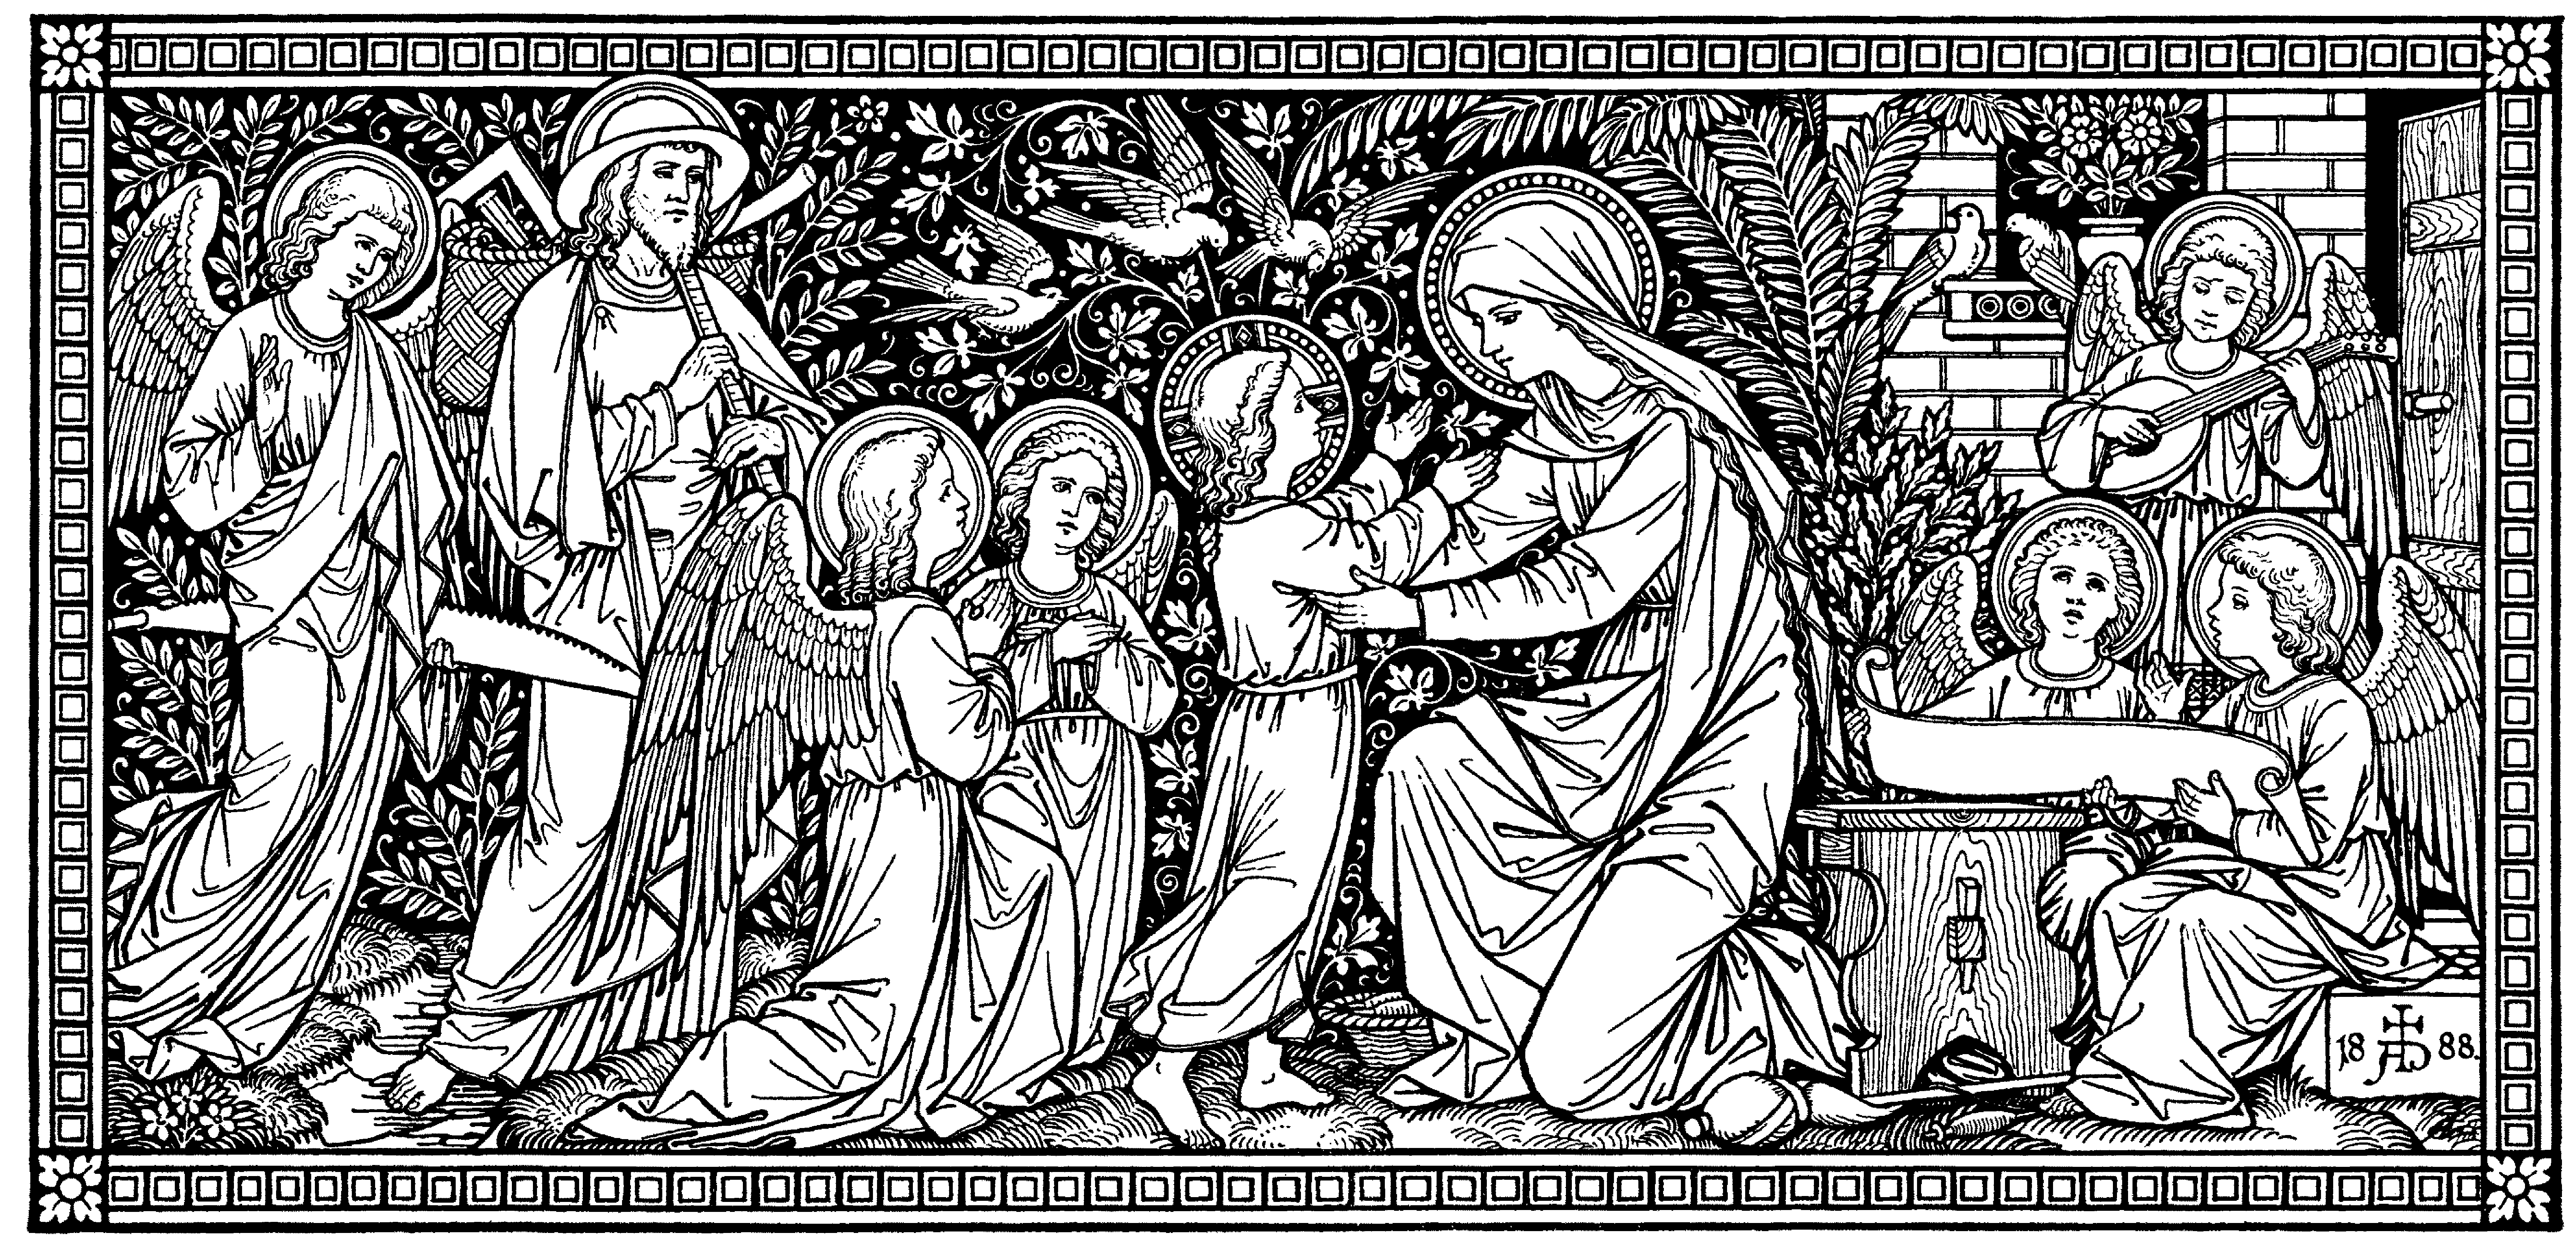
\includegraphics[height=5.5cm]{images/SainteFamille}
\end{center}

\newpage

\vspace*{1cm}
\titre{\selectfont\lettrinesD{La Messe de Mariage}}

\titre{%
Prières au bas de l'autel}

\rubrique{Le prêtre et les ministres qui l'assistent se préparent à la célébration de la Liturgie par les prières dites au bas de l'autel. À la messe chantée elles sont dites à voix basse ; on se reporte directement à l'Introït.}

\traduire{%
In nómine Patris, et Fílii, et Spíritus Sancti. Amen.}{%
Au nom du Père, et du Fils, et du Saint-Esprit. Ainsi soit-il.}

\traduire{%
\V~Introíbo ad altáre Dei.}{%
\V~Je monterai à l'autel de Dieu.}

\traduire{%
\R~\textbf{Ad Deum, qui lætíficat iuventútem meam.}}{%
\R~\textbf{Jusqu'au Dieu qui réjouit ma jeunesse.}}

\traduire{%
\V~Iúdica me, Deus, et discérne causam meam de gente non sancta : ab hómine iníquo et dolóso érue me.}{%
\V~Jugez-moi, ô Dieu, et distinguez ma cause de celle de la nation impie : arrachez-moi de l'homme inique et trompeur.}

\traduire{%
\R~\textbf{Quia tu es, Deus, fortitúdo mea : quare me repulísti, et quare tristis incédo, dum afflígit me inimícus ?}}{%
\R~\textbf{Car, ô Dieu, vous êtes ma force : pourquoi m'avez-vous repoussé, et pourquoi m'en vais-je triste, tandis que l'ennemi m'afflige ?}}

\traduire{%
\V~Emítte lucem tuam et veritátem tuam : ipsa me deduxérunt et adduxérunt in montem sanctum tuum, et in tabernácula tua.}{%
\V~Envoyez votre lumière et votre vérité : elles m'ont conduit et m'ont amené à votre montagne sainte et dans vos palais.}

\traduire{%
\R~\textbf{Et introíbo ad altáre Dei : ad Deum qui lætíficat iuventútem meam.}}{%
\R~\textbf{Et je monterai à l'autel de Dieu, jusqu'au Dieu qui réjouit ma jeunesse.}}

\traduire{%
\V~Confitébor tibi in cíthara, Deus, Deus meus : quare tristis es anima mea, et quare contúrbas me ?}{%
\V~Je vous louerai sur la harpe, ô Dieu, mon Dieu : pourquoi es-tu triste, ô mon âme, et pourquoi me troubles-tu ?}

\traduire{%
\R~\textbf{Spera in Deo, quóniam adhuc confitébor illi : salutáre vultus mei, et Deus meus.}}{%
\R~\textbf{Espère en Dieu, parce que je le louerai encore : il est le salut de mon visage et il est mon Dieu.}}

\traduire{%
\V~Glória Patri, et Fílio, et Spirítui Sancto.}{%
\V~Gloire au Père, et au Fils, et au Saint-Esprit.}

\traduire{%
\R~\textbf{Sicut erat in princípio, et nunc, et semper : et in s\'æcula sæculórum. Amen.}}{%
\R~\textbf{Comme il était au commencement, maintenant, et toujours, et dans les siècles des siècles. \ainsi.}}

\traduire{%
\V~Introíbo ad altáre Dei.}{%
\V~Je monterai à l'autel de Dieu.}

\traduire{%
\R~\textbf{Ad Deum qui lætíficat iuventútem meam.}}{%
\R~\textbf{Jusqu'au Dieu qui réjouit ma jeunesse.}}

\traduire{%
\V~Adiutórium~\x\ nostrum in nómine Dómini.}{%
\V~Notre~\x\ secours est dans le nom du Seigneur.}

\traduire{%
\R~\textbf{Qui fecit cælum et terram.}}{%
\R~\textbf{Qui a fait le ciel et la terre.}}

\rubrique{%
Le célébrant récite le \emph{Confiteor}, puis les ministres (et les fidèles à la messe lue) répondent :%
}
\traduire{%
\V~Misereátur tui omnípotens Deus, et dimissis peccátis tuis, perdúcat te ad vitam ætérnam.}{%
\V~Que le Dieu tout-puissant vous fasse miséricorde, vous pardonne vos péchés, et vous conduise à la vie \mbox{éternelle.}}

\traduire{%
\R~\textbf{Amen.}}{%
\R~\textbf{Ainsi soit-il.}}

\medskip
\rubrique{%
Les ministres récitent alors le \emph{Confiteor} :%
}
\label{Confiteor}\traduire{%
Confíteor Deo omnipoténti, beátæ Maríæ semper Vírgini, beáto Michaéli Archángelo, beáto Ioánni Baptístæ, sanctis Apóstolis Petro et Páulo, ómnibus Sanctis, et tibi pater : quia peccávi nimis cogitatióne, verbo, et ópere : mea culpa, mea culpa, mea máxima culpa. Ideo precor beátam Maríam semper Vírginem, beátum Michaélem Archángelum, beátum Ioánnem Baptístam, sanctos Apóstolos Petrum et Páulum, omnes Sanctos, et te, pater, oráre pro me ad Dóminum Deum nostrum.}{%
Je confesse à Dieu tout-puissant, à la bienheureuse Marie toujours vierge, à saint Michel Archange, à saint Jean-Baptiste, aux saints Apôtres Pierre et Paul, à tous les saints et à vous mon père, que j'ai beaucoup péché, par pensées, par paroles et par actions. C'est ma faute, c'est ma faute, c'est ma très grande faute. C'est pourquoi je supplie la bienheureuse Marie toujours vierge, saint Michel Archange, saint Jean-Baptiste, les saints Apôtres Pierre et Paul, tous les saints et vous mon père, de prier pour moi le Seigneur notre Dieu.}

\medskip

\traduire{%
\V~Misereátur vestri omnípotens Deus, et dimíssis peccátis vestris, perdúcat vos ad vitam ætérnam.}{%
\V~Que le Dieu tout-puissant vous fasse miséricorde, qu'il vous pardonne vos péchés et vous conduise à la vie éternelle.}

\traduire{%
\R~\textbf{Amen.}}{%
\R~\textbf{Ainsi soit-il.}}

\traduire{%
Indulgéntiam,~\x\ absolutiónem, et remissiónem peccatórum nostrórum, tríbuat nobis omnípotens et miséricors Dóminus.}{%
Que le Dieu tout-puissant et miséricordieux nous accorde le pardon,~\x\  l'absolution et la rémission de nos péchés.}

\traduire{%
\R~\textbf{Amen.}}{%
\R~\textbf{Ainsi soit-il.}}

\traduire{%
\V~Deus, tu convérsus vivificábis nos.}{%
\V~Dieu, tournez-vous vers nous et donnez-nous la vie.}

\traduire{%
\R~\textbf{Et plebs tua lætábitur in te.}}{%
\R~\textbf{Votre peuple se réjouira en vous.}}

\traduire{%
\V~Osténde nobis Dómine, misericórdiam tuam.}{%
\V~Montrez-nous, Seigneur, votre miséricorde.}

\traduire{%
\R~\textbf{Et salutáre tuum da nobis.}}{%
\R~\textbf{Accordez-nous votre salut.}}

\traduire{%
\V~Dómine, exáudi oratiónem meam.}{%
\V~Seigneur, exaucez ma prière.}

\traduire{%
\R~\textbf{Et clamor meus ad te véniat.}}{%
\R~\textbf{Que mon appel vous parvienne.}}

\traduire{%
\V~Dóminus vobíscum.}{%
\V~Le Seigneur soit avec vous.}

\traduire{%
\R~\textbf{Et cum spíritu tuo.}}{%
\R~\textbf{Et avec votre esprit.}}

\traduire{%
Orémus.}{%
Prions.}

\rubrique{En montant à l'autel le prêtre dit la prière suivante :}



\traduire{%
Aufer a nobis, qu\'æsumus, Dómine, iniquitátes nostras : ut ad Sancta sanctórum puris mereámur méntibus introíre. Per Christum Dóminum nostrum. Amen.}{%
Enlevez nos fautes, Seigneur, pour que nous puissions pénétrer dans le Saint des Saints avec une âme pure. Par le Christ notre Seigneur. Ainsi soit-il.}


\rubrique{L'autel, en pierre, représente le Christ : \emph{il est la pierre vivante choisie par Dieu} (I~Pierre, 2,4). Cette pierre contient les reliques des martyrs qui ont versé leur sang pour le Christ. En la baisant le prêtre adore le Christ et vénère les saints martyrs.}


\traduire{%
Orámus te, Dómine, per mérita Sanctórum tuórum, quorum relíquiæ hic sunt, et ómnium Sanctórum : ut indúlgere dignéris ómnia peccáta mea. Amen.}{%
Nous vous en prions, Seigneur, par les mérites de vos saints (il baise l'autel au milieu) dont nous avons ici les reliques et de tous les saints, daignez pardonner tous mes péchés. Ainsi soit-il.}

\rubrique{Le Célébrant, avant de lire l'antienne d'Introït, bénit l'encens, en disant :}
\traduire{%
Ab illo bene\x dicáris, in cuius honóre cremáberis. Amen.}{%
Sois bé\x ni par celui en l'honneur de qui tu vas brûler. Ainsi soit-il.}

\rubrique{Et ayant reçu l'encensoir du diacre, il encense l'autel, sans rien dire. Puis le diacre, ayant reçu l'encensoir du Prêtre, encense ce dernier.}

\titre{\selectfont\lettrinesE{Avant-messe}}

\rubrique{La première partie de la Liturgie est appelée "Avant-messe" ou "messe des catéchumènes". Elle est une préparation au saint Sacrifice et consiste dans un ensemble de prières, de chants et de lectures de la Sainte \'Ecriture. Chaque jour liturgique a un thème ou une orientation spirituelle particulière qui y est exprimée. \emph{Les chants sacrés qui résument les plus saintes vérités préparent harmonieusement nos âmes aux mystères que nous devons célébrer. Ils nous mettent à l'unisson des chants divins et nous accordent aux réalités divines, avec nous-mêmes et les uns aux autres : nous ne formons plus qu'un ch\oe ur unique et homogène d'hommes saints}. (Denys l'Aréopagite)}

\titre{Introït}
\traduire{Deus Israël coniungat vos : et ipse sit vobiscum, qui misertus est duobus unicis : et nunc, Domine, fac eos plenius benedicere te. \V Beati omnes qui timent Dominum : qui ambulant in viis eius.}{Que le Dieu d'Israël vous unisse et qu'il reste avec vous, lui qui a eu pitié de deux enfants uniques ! Et maintenant, Seigneur, faites qu'ils reconnaissent de plus en plus vos bontés. Alléluia, alléluia. \V~Heureux tous ceux qui craignent le Seigneur, et qui marchent dans ses voies. Gloire au Père.}



\titre{Kyrie}
\rubrique{Le Kyrie est le reste d'une litanie plus longue, qui était toujours chantée en grec. Le diacre formulait des intentions et on répondait : Seigneur, ayez pitié. De cette litanie il ne reste aujourd'hui que neuf invocations, trois pour chaque personne de la Sainte Trinité. Nous recommandons à Dieu les besoins de l'Eglise et nos intentions personnelles.}

\traduire{Kyrie eleison \emph{(ter)}}{Seigneur ayez pitié de nous \emph{(ter)}}
\traduire{Christe eleison \emph{(ter)}}{Christ ayez pitié de nous \emph{(ter)}}
\traduire{Kyrie eleison \emph{(ter)}}{Seigneur ayez pitié de nous \emph{(ter)}}


\titre{Gloria}
\rubrique{Le Gloria faisait partie de l'office de nuit et fut progressivement introduit dans la messe à partir du V\ieme\ siècle. C'est un développement du chant des anges dans la nuit de Noël. C'est la grande glorification du Dieu trinitaire : Gloire au Père, au Fils et au Saint-Esprit.}

\traduire{%
Glória in excélsis Deo. Et in terra pax homínibus bonæ voluntátis. Laudámus te. Benedícimus te. Adorámus te. Glorificámus te. Grátias ágimus tibi propter magnam glóriam tuam. Dómine Deus, Rex c\oe léstis, Deus Pater omnípotens. Dómine Fili unigénite, Jesu Christe. Dómine Deus, Agnus Dei, Fílius Patris. Qui tollis peccáta mundi, miserére nobis. Qui tollis peccáta mundi, súscipe deprecatiónem nostram. Qui sedes ad déxteram Patris, miserére nobis. Quóniam tu solus Sanctus. Tu solus Dóminus. Tu solus Altíssimus, Jesu Christe. Cum Sancto Spíritu in glória Dei Patris. Amen.%
}{%
Gloire à Dieu au plus haut des cieux, et paix sur la terre aux hommes de bonne volonté. Nous vous louons, nous vous bénissons, nous vous adorons, nous vous glorifions. Nous vous rendons grâces pour votre gloire immense, Seigneur Dieu, Roi du ciel, Dieu Père tout-puissant. Seigneur Fils unique, Jésus-Christ, Seigneur Dieu, Agneau de Dieu, Fils du Père, vous qui enlevez les péchés du monde, ayez pitié de nous ; vous qui enlevez les péchés du monde, accueillez notre prière ; vous qui siégez à la droite du Père, ayez pitié de nous. Car vous êtes le seul Saint, le seul Seigneur, le seul Très-Haut, Jésus-Christ, avec le Saint-Esprit, dans la gloire de Dieu le Père. \ainsi.%
}%

\titre{Collecte}
\rubrique{Le prêtre se tourne vers les fidèles pour les saluer et les inviter à s'unir à la prière qu'il va prononcer en leur nom.}


\traduire{%
\V~Dóminus vobíscum.}{%
\V~Le Seigneur soit avec vous.}

\traduire{%
\R~\textbf{Et cum spíritu tuo.}}{%
\R~\textbf{Et avec votre esprit.}}

\rubrique{La Collecte chantée par le prêtre exprime l'intention de la prière de l'Église en ce jour et la grâce spéciale qu'elle demande. Cette oraison est répétée plusieurs fois au cours de l'office. Le prêtre la prononce les mains élevées comme pour diriger la prière vers le ciel ; dans la Sainte Écriture élever les mains est synonyme de prier. On se tient debout, sauf les jours de pénitence et aux messes des défunts, où l'on est à genoux.}

\traduire{%
Orémus.}{%
Prions.}
\traduire{%
Exáudi nos, omnípotens et miséricors Deus~: ut, quod nostro ministrátur offício, tua benedictióne pótius impleátur. Per Dóminum nostrum Iesum Christum Fílium tuum, qui tecum vivit et regnat in unitáte Spíritus Sancti Deus, per ómnia s\'\ae cula sæculórum. \\
\R~\textbf{Amen.}}{%
Écoutez-nous, Dieu tout-puissant et miséricordieux~: que votre bénédiction donne son plein achèvement à ce que nous venons d'accomplir en vertu de notre charge. Par Notre Seigneur Jésus-Christ votre Fils, qui étant Dieu vit et règne avec vous en l'unité du Saint-Esprit, dans tous les siècles des siècles. \\ 
\R~\textbf{\ainsi.}}
\vspace*{0.5cm}
\titre{Épître}

\rubrique{Les lectures ne suivent pas l'ordre des livres de la Bible, mais l'Église a choisi les textes les plus importants en rapport avec le temps liturgique ou le mystère célébré en ce jour.}
\traduire{%
Léctio Epístolæ beáti Pauli Apóstoli ad Ephésios.

Fratres~: Mulíeres viris suis súbditæ sint, sicut Dómino~: quóniam vir caput est mulíeris~: sicut Christus caput est Ecclésiæ~: Ipse, salvátor córporis eius. Sed, sicut Ecclésia subiécta est Christo, ita et mulíeres viris suis in ómnibus.
Viri, dilígite uxóres vestras, sicut et Christus diléxit Ecclésiam, et seípsum trádidit pro ea, ut illam sanctificáret, mundans lavácro aquæ in verbo vitæ, ut exhibéret ipse sibi gloriósam Ecclésiam, non habéntem máculam, aut rugam, aut áliquid huiúsmodi, sed ut sit sancta et immaculáta. Ita et viri debent dilígere uxóres suas, ut córpora sua. Qui suam uxórem díligit, seípsum díligit. Nemo enim unquam carnem suam ódio hábuit~: sed nutrit, et fovet eam, sicut et Christus Ecclésiam~: quia membra sumus córporis eius, de carne eius, et de óssibus eius.
Propter hoc relínquet homo patrem et matrem suam, et adhærébit uxóri suæ~: et erunt duo in carne una. Sacraméntum hoc magnum est, ego autem dico in Christo, et in Ecclésia. Verúmtamen et vos sínguli, unusquísque uxórem suam, sicut seípsum díligat~: uxor autem tímeat virum suum.\\
}{%
Lecture de l'Épître de Saint Paul aux Éphésiens.

Frères, que les femmes soient soumises à leur mari comme au Seigneur~; car le mari est le chef de la femme comme le Christ est le Chef de l'Église, qui est son Corps et dont il est le Sauveur. De même donc que l'Église est soumise au Christ, que les femmes le soient aussi à leur mari en toutes choses.
Vous, maris, aimez vos femmes tout comme le Christ a aimé l'Église et s'est livré pour elle, afin de la sanctifier en la purifiant par le baptême et la parole de vie~; il s'est ainsi préparé une Église resplendissante, sans tache, ni ride, ni rien de tel, mais sainte et irréprochable. Ainsi, les maris doivent aimer leur femme comme leur propre corps. Qui aime sa femme s'aime lui-même. Personne n'a jamais haï sa propre chair, mais il la nourrit et la soigne tout comme le Christ fait pour l'Église, puisque nous sommes les membres de son corps, formés de sa chair et de ses os.
C'est pourquoi l'homme quittera son père et sa mère pour s'attacher à sa femme, et les deux ne feront qu'une seule chair. Quel grand mystère~! Je veux dire par rapport au Christ et à l'Église. Ainsi donc, que chacun de vous aime sa femme comme soi-même, et que la femme ait pour son mari un affectueux respect.\\
}
\traduire{%
\R~\textbf{Deo gratias}}{%
\R \textbf{Rendons grâces à Dieu}}

\titre{Graduel}
\rubrique{Graduel, Alléluia sont des chants de méditation sur les lectures ou le mystère liturgique de ce jour. \emph{Alleluia} signifie "louez Dieu". L'Alléluia se prolonge dans une mélodie ornée qui exprime la joie spirituelle au-delà des paroles. C'est pourquoi le Graduel est remplacé au temps pascal par un deuxième Alléluia, alors que le Trait remplace l'Alléluia depuis la Septuagésime jusqu'à Pâques.}

\traduire{Uxor tua sicut vitis abundans in lateribus domus tuae. \V Filii tui sicut novellae olivarum in circuitu mensae tuae}{Ton épouse sera comme une treille chargée de grappes sur les murs de ta maison. \V Tes enfants, autour de la table, comme des jeunes pousses d'olivier.}

\titre{Alléluia}
\traduire{Alleluia, Alleluia. \V Mittat vobis Dominus auxilium de sancto : et de Sion tueatur vos. Alleluia.}{Alléluia, Dieu soit loué ! Que le Seigneur vous envoie du secours de son temple saint ; et qu'il vous protège du haut de la colline de Sion.}

\titre{Évangile}

\rubrique{On chante le saint Évangile tourné vers le Nord (le ch\oe ur étant normalement orienté vers l'Est) parce que le Nord symbolise les âmes qui se trouvent dans la froideur de l'infidélité et de l'ignorance du Christ, et qui sont éveillées par le souffle du Saint-Esprit.}


\traduire{%
\x~Sequéntia sancti Evangélii secúndum Matth\'\ae um.

In illo témpore~: Accessérunt ad Iesum pharis\'\ae i tentántes eum, et dicéntes~: Si licet hómini dimíttere uxórem suam quacúmque ex causa~? Qui respóndens, ait eis~: Non legístis, quia qui fecit hóminem ab inítio, másculum et féminam fecit eos~? et dixit~: Propter hoc dimíttet homo patrem, et matrem, et adhærébit uxóri suæ, et erunt duo in carne una. Itaque iam non sunt duo, sed una caro. Quod ergo Deus coniúnxit, homo non séparet.}{%
\x~Suite du saint Évangile selon Saint Matthieu.

En ce temps-là, des pharisiens s'approchèrent de Jésus, et pour l'embarrasser lui dirent~: \og Est-il permis à un homme de répudier sa femme pour n'importe quel motif~? N'avez-vous donc pas lu, répondit Jésus, que le Créateur, à l'origine, fit l'homme et la femme~? et qu'il a dit~: \emph{C'est pourquoi l'homme quittera son père et sa mère pour s'attacher à sa femme, et les deux ne seront qu'une seule chair}. Désormais, ils ne seront plus deux, mais ils seront un seul corps. Et par suite, ce que Dieu a uni, l'homme ne peut le séparer.\fg}
\newpage
\titre{%
Credo%
}


\traduire{%
Credo in Deum, Patrem omnipoténtem, factórem caeli et terrae, visibilium omnium et invisibilium.\\
Et in unum Dóminum Iesum Christum, Fílium Dei unigenitum. Et ex Patre natum ante ómnia s\'\ae cula. Deum de Deo, lumen de lúmine, Deum verum de Deo vero. Génitum, non factum, consubstantiálem Patri: per quem ómnia facta sunt. Qui propter nos hómines et propter nostram salútem descéndit de cælis. Et incarnátus est de Spíritu Sancto ex María Vírgine: et homo factus est. Crucifíxus étiam pro nobis: sub Póntio Piláto passus, et sepúltus est. Et resurréxit tértia die, secúndum Scriptúras. Et ascéndit in caelum: sedet ad déxteram Patris. Et iterum ventúrus est cum glória iudicáre vivos et mórtuos: cuius regni non erit finis.\\
Et in Spíritum Sanctum, Dóminum, et vivificántem: qui ex Patre Filióque procédit. Qui cum Patre et Fílio simul adorátur et conglorificátur: qui locútus est per Prophétas.\\
Et unam sanctam cathólicam et apostólicam Ecclésiam. Confíteor unum baptísma in remissiónem peccatórum. Et exspécto resurrectiónem mortuórum. Et vitam ventúri s\'\ae culi. Amen.%
}{%
  Je crois en un seul Dieu, le Père tout-puissant, créateur du ciel et de la terre, de toutes choses, visibles et invisibles.\\
  Je crois en un seul Seigneur Jésus-Christ, le Fils unique de Dieu, né du Père avant tous les siècles ; Dieu né de Dieu, lumière née de la lumière, vrai Dieu né du vrai Dieu. Engendré, non pas créé, consubstantiel au Père, et par qui tout a été créé. C'est lui qui, pour nous les hommes, et pour notre salut, est descendu des cieux. Il a pris chair de la Vierge Marie par l'action du Saint-Esprit, et il s'est fait homme. Puis il fut crucifié pour nous sous Ponce-Pilate : il souffrit et fut mis au tombeau. Il ressuscita le troisième jour, suivant les Ecritures. Il monta aux cieux, où il siège à la droite du Père. De nouveau il viendra dans la gloire pour juger les vivants et les morts, et son règne n'aura pas de fin.\\
  Je crois en l'Esprit-Saint, qui est Seigneur et qui donne la vie, qui procède du Père et du Fils. Avec le Père et le Fils, il reçoit même adoration et même gloire. Il a parlé par les prophètes.\\
  Je crois à l'Église une, sainte, catholique et apostolique. Je reconnais un seul Baptême pour la rémission des péchés, et j'attends la résurrection des morts et la vie du monde à venir. \ainsi.
}


\newpage
\titre{\selectfont\lettrinesE{Offertoire}}

\begin{center}
\includegraphics[height=5.7cm]{images/offertoires20}
\end{center}


\rubrique{À l'Offertoire l'Église offre le Corps et le Sang du Christ, représentés par le pain et le vin. Notre Seigneur a communiqué à son Église le pouvoir d'offrir le même sacrifice qu'il offrit sur la Croix. L'Église s'y unit comme victime. \emph{Le Christ lui-même est à la fois le prêtre qui offre et la victime qui est offerte. Le sacrifice de l'Église est le sacrement quotidien du sacrifice du Christ. L'Église, qui est le corps dont il est la tête, s'y offre elle-même par lui. C'est pourquoi dans ce sacrement l'Église elle-même est offerte dans ce qu'elle offre.} (S.~Augustin). Nous sommes donc une seule victime avec le Christ, unissant nos propres offrandes et nos sacrifices à celui du Christ et de l'Église. Notre participation à cette offrande est exprimée par le chant de l'offertoire.}


\traduire{%
\V~Dóminus vobíscum.}{%
\V~Le Seigneur soit avec vous.}

\traduire{%
\R~\textbf{Et cum spíritu tuo.}}{%
\R~\textbf{Et avec votre esprit.}}

\traduire{%
Orémus.}{%
Prions.}
\traduire{In te speravi, Domine : dixi : Tu es Deus meus : in manibus tuis tempora mea.}{En vous, Seigneur, je mets toute ma confiance ; aussi ai-je dit : Vous êtes mon Dieu, ma destinée est entre vos mains.}

\titre{%
Offrande du pain}

\traduire{%
  Súscipe, sancte Pater, omnípotens ætérne Deus, hanc immaculátam hóstiam, quam ego indígnus fámulus tuus óffero tibi Deo meo, vivo et vero, pro innumerabílibus peccátis, et offensiónibus, et negligéntiis meis, et pro ómnibus circumstántibus, sed et pro ómnibus fidélibus christiánis vivis atque defúnctis : ut mihi et illis profíciat ad salútem in vitam ætérnam. Amen.}{%
  Recevez, Père saint, Dieu éternel et tout-puissant, cette offrande sans tache, que moi, votre indigne serviteur, je vous présente, à vous, mon Dieu vivant et vrai, pour mes péchés, offenses et négligences sans nombre, pour tous ceux qui m'entourent, ainsi que pour tous les fidèles vivants et morts : qu'elle serve à mon salut et au leur pour la vie éternelle. \ainsi.}

\titre{%
Préparation et offrande du vin}

\noindent\parbox{\textwidth}{%
%
\rubrique{%
  Le Diacre prépare le calice en y versant le vin ; le sous-Diacre y ajoute quelques gouttes d'eau que le Célébrant bénit. L'eau mêlée au vin figure l'union en Jésus-Christ de la nature humaine à la personne divine, et symbolise aussi le chrétien intimement uni au Christ. Le vin et l'eau rappellent le sang et l'eau qui coulèrent du côté du Christ percé par la lance. \emph{Quand le vin et l'eau sont mêlés dans le calice, le peuple est uni au Christ et la foule des croyants est associée et réunie à celui en qui elle croit.} \mbox{(S. Cyprien)}}%
%
}

\traduire{%
  Deus,~\x\ qui humánæ substántiæ dignitátem mirabíliter condidísti, et mirabílius reformásti : da nobis, per huius aquæ et vini mystérium, eius divinitátis esse consórtes, qui humanitátis nostræ fíeri dignátus est párticeps, Iesus Christus, Fílius tuus, Dóminus noster : Qui tecum vivit et regnat in unitáte Spíritus Sancti Deus : per ómnia saécula sæculórum. Amen.}{%
  Dieu,~\x\ qui, d'une manière admirable, avez créé la nature humaine dans sa noblesse, et l'avez restaurée d'une manière plus admirable encore, accordez-nous, selon le mystère de cette eau et de ce vin, de prendre part à la divinité de celui qui a daigné partager notre humanité, Jésus-Christ votre Fils, notre Seigneur, qui, étant Dieu, vit et règne avec vous en l'unité du Saint-Esprit, dans tous les siècles des siècles. \ainsi.}

\traduire{%
  Offérimus tibi, Dómine, cálicem salutáris, tuam deprecántes cleméntiam : ut in conspéctu divínæ maiestátis tuæ, pro nostra et totíus mundi salúte, cum odóre suavitátis ascéndat. Amen.}{%
  Nous vous offrons, Seigneur, le calice du salut, et nous demandons à votre clémence qu'il s'élève en parfum agréable devant votre divine Majesté, pour notre salut et celui du monde entier. \ainsi.}

\traduire{%
  In spíritu humilitátis, et in ánimo contríto suscipiámur a te, Dómine : et sic fiat sacrifícium nostrum in conspéctu tuo hódie, ut pláceat tibi, Dómine Deus.}{%
  Voyez l'humilité de nos âmes et la contrition de nos c\oe urs : accueillez-nous, Seigneur, et que notre sacrifice s'accomplisse aujourd'hui devant vous de telle manière qu'il vous soit agréable, Seigneur Dieu.}

\traduire{%
  Veni, sanctificátor, omnípotens ætérne Deus : et béne\x dic hoc sacrifícium, tuo sancto nómini præparátum.}{%
  Venez, Sanctificateur, Dieu éternel et tout-puissant, et bé\x nissez ce sacrifice préparé pour votre saint Nom.}


\noindent\parbox{\textwidth}{%
%
\titre{%
Encensement}

\rubrique{%
  Comme l'encens, consumé par le feu, s'élève en vapeur odorante, ainsi l'Église avec le Christ, consumée par le feu du Saint-Esprit, s'élève en sacrifice envers Dieu. On encense les oblats (le pain et le vin), puis l'autel, le Célébrant, et enfin le clergé et les fidèles.}%
%
}

\traduire{%
  Per intercessiónem beáti Michaélis archángeli, stantis a dextris altáris incénsi, et ómnium electórum suórum, incénsum istud dignétur Dóminus bene\x dícere, et in odórem suavitátis accípere. Per Christum Dóminum nostrum. Amen.}{%
  Par l'intercession de l'archange saint Michel, qui se tient à droite de l'autel de l'encens, et par l'intercession de tous ses élus, que le Seigneur daigne bé\x nir cet encens, et le recevoir comme un parfum agréable. Par le Christ notre Seigneur. \ainsi.}

\traduire{%
  Incénsum istud, a te benedíctum, ascéndat ad te, Dómine : et descéndat super nos misericórdia tua. }{%
  Que cet encens béni par vous, Seigneur, monte vers vous, et que descende sur nous votre miséricorde.}

\traduire{%
  Dirigátur, Dómine, orátio mea, sicut incénsum, in conspéctu tuo : elevátio mánuum meárum sacrifícium vespertínum. Pone, Dómine, custódiam ori meo, et óstium circumstántiæ lábiis meis : ut non declínet cor meum in verba malítiæ, ad excusándas excusatiónes in peccátis.}{%
  Seigneur, que ma prière s'élève comme l'encens devant votre face ; que mes mains levées soient comme l'offrande du soir. Placez, Seigneur, une garde à ma bouche et une barrière tout autour de mes lèvres. Que mon c\oe ur ne se porte pas à des paroles mauvaises qui servent de prétexte au péché. (Ps.~140)}

\traduire{%
  Accéndat in nobis Dóminus ignem sui amóris, et flammam ætérnæ caritátis. Amen.}{%
  Que le Seigneur allume en nous le feu de son amour et la flamme de l'éternelle charité. \ainsi.}

%\vfill\pagebreak[1]

\noindent\parbox{\textwidth}{%
%
\titre{%
Lavabo}

\rubrique{%
  \emph{%
  Les mains sont le symbole de l'action. En les lavant nous signifions la pureté et l'innocence des actions.} (S.Cyprien)}%
%
}

\traduire{%
  Lavábo inter innocéntes manus meas : et circúmdabo altáre tuum, Dómine : Ut áudiam vocem laudis, et enárrem univérsa mirabília tua. Dómine, diléxi decórem domus tuæ, et locum habitatiónis glóriæ tuæ. Ne perdas cum ímpiis, Deus, ánimam meam, et cum viris sánguinum vitam meam : In quorum mánibus iniquitátes sunt : déxtera eórum repléta est munéribus. Ego autem in innocéntia mea ingréssus sum : rédime me, et miserére mei. Pes meus stetit in dirécto : in ecclésiis benedícam te, Dómine. Glória Patri, et Fílio, et Spirítui Sancto, Sicut erat in princípio, et nunc, et semper, et in saécula sæculórum. Amen.}{%
  Je laverai mes mains parmi les innocents, et je me tiendrai devant votre autel, Seigneur. Pour entendre la voix de la louange et raconter toutes vos merveilles. Seigneur, j'aime la beauté de votre maison et le lieu où réside votre gloire. Ô Dieu, ne condamnez pas mon âme avec celle des impies ; ne m'enlevez pas la vie comme aux hommes de sang. Leurs mains commettent l'iniquité, et leur droite est comblée de présents. Pour moi je marche dans l'innocence ; rachetez-moi et ayez pitié de moi. Mon pied se tient dans la voie droite ; je vous bénirai, Seigneur, dans l'assemblée. Gloire au Père, au Fils, et au Saint-Esprit. Comme il était au commencement, maintenant et toujours, et dans tous les siècles des siècles. \ainsi.}

\titre{%
Prière à la Sainte Trinité}

\traduire{%
  Súscipe, sancta Trínitas, hanc oblatiónem, quam tibi offérimus ob memóriam passiónis, resurrectiónis, et ascensiónis Iesu Christi Dómini nostri : et in honórem beátæ Maríæ semper Vírginis, et beáti Ioánnis Baptístæ, et sanctórum Apostolórum Petri et Pauli, et istórum, et ómnium sanctórum : ut illis profíciat ad honórem, nobis autem ad salútem : et illi pro nobis intercédere dignéntur in cælis, quorum memóriam ágimus in terris. Per eúndem Christum Dóminum nostrum. Amen.}{%
  Recevez, Trinité Sainte, cette offrande que nous vous présentons en mémoire de la Passion, de la Résurrection et de l'Ascension de Jésus-Christ notre Seigneur, en l'honneur aussi de la bienheureuse Marie toujours vierge, de saint Jean-Baptiste, des saints Apôtres Pierre et Paul, des saints dont les reliques sont ici, et de tous les saints. Qu'elle soit pour eux une source d'honneur, et pour nous une cause de salut, et qu'ils daignent intercéder pour nous au ciel, eux dont nous célébrons la mémoire sur terre. Par le Christ notre Seigneur. \ainsi.}

\traduire{%
  Oráte, fratres : ut meum ac vestrum sacrifícium acceptábile fiat apud Deum Patrem omnipoténtem}{%
  Priez, mes frères, pour que mon sacrifice, qui est aussi le vôtre, puisse être agréé par Dieu le Père tout-puissant.}

\rubrique{%
  On répond :}

\traduire{%
\R~\textbf{Suscípiat Dóminus sacrifícium de mánibus tuis, ad laudem et glóriam nóminis sui, ad utilitátem quoque nostram, totiúsque Ecclésiæ suæ sanctæ.}}{%
\R~\textbf{Que le Seigneur reçoive de vos mains le sacrifice, à la louange et à la gloire de son Nom, ainsi que pour notre bien et celui de toute sa sainte Église.}}

\titre{%
Secrète}

\rubrique{%
  L'oraison secrète donne l'intention spéciale du sacrifice du jour.}
\traduire{%
Súscipe, qu\'\ae sumus, Dómine, pro sacra connúbii lege munus oblátum~: et, cuius largítor es óperis, esto dispósitor. Per Dóminum nostrum Iesum Christum Fílium tuum, qui tecum vivit et regnat in unitáte Spíritus Sancti Deus,}{%
Recevez, Seigneur, l'offrande que nous vous présentons en raison du caractère sacré du lien conjugal~; et présidez à cette union dont vous êtes l'auteur. Par Notre Seigneur Jésus-Christ votre Fils, qui étant Dieu vit et règne avec vous en l'unité du Saint-Esprit,}

\traduire{%
\V~\Peromnia.}{%
\V~\Siecles.}
\rubrique{%
  On répond :}

\traduire{%
\R~\textbf{Amen.}}{%
\R~\textbf{\ainsi.}}


\titre{%
Oblation du Sacrifice}

\rubrique{%
  Commence ici la partie la plus sacrée de la Liturgie : le sacrifice réel et sacramentel où le Prêtre immole le Christ. \emph{Vraiment à cette heure très redoutable il faut tenir haut son c\oe ur vers Dieu, et non en bas vers la terre et les affaires terrestres. D'autorité donc le Célébrant  enjoint à cette heure à tous de laisser de côté les soucis, les sollicitudes domestiques, et de tenir leur c\oe ur au ciel vers Dieu ami des hommes.} (S.Cyrille de Jérusalem)}

\titre{%
Préface}

\rubrique{%
  Par le chant de la Préface, le Célébrant rend grâces à Dieu au nom de l'Église pour l'\oe uvre du salut réalisée par Jésus-Christ.}
\introprefacetraduite

%\enlargethispage{\baselineskip}
\traduire{%
  Vere dignum et iustum est, \'æquum et salutáre,nos tibi semper et ubique gratias agere, Domine sancte Pater, Omnipotens \ae terne Deus : Per Christum Dominum Nostrum. Per quem maiestatem tuam laudant angeli, adorant Dominationes, tremunt Potestates. C\ae li c\ae lorumque Virtutes, ac beata Seraphim, socia exultatione concelebrant. Cum quibus et nostras voces, ut admitti iubeas, deprecamur supplici confessione dicentes :}{%
  Il est vraiment digne et juste, équitable et salutaire, de vous rendre grâce toujours et partout, Seigneur, Père Saint, Dieu éternel et Tout-Puissant, par le Christ Notre-Seigneur. Par lui les anges louent votre majesté, les Dominations l'adorent, les Puissances la révèresnt, les Cieux et les Forces des Cieux, avec les bienheureux Séraphins, la célèbrent, unis dans une même allégresse. A leurs chants, nous vous prions de laisser se joindre aussi nos voix, pour proclamer dans une humble louange : }


\titre{%
Sanctus}

\rubrique{%
  L'hymne au Dieu trois fois saint se compose d'une vision du prophète Isaïe (Is. 6,3) et des acclamations chantées lors de l'entrée triomphale du Christ à Jérusalem. Le sacrifice du Christ s'achève par sa résurrection et son ascension : Notre-Seigneur entre triomphalement dans la Jérusalem céleste. \emph{Le Christ est entré une fois pour toutes dans le sanctuaire du ciel avec son propre sang, nous ayant acquis une rédemption éternelle.} (Hébreux,9,12). \emph{Nous chantons cette glorification qui nous a été transmise des Séraphims, pour que, en communiant  à cette hymne, nous soyons unis aux armées angéliques.} \mbox{(S. Cyrille de Jérusalem)}}

\traduire{%
Sanctus, sanctus, sanctus Dóminus, Deus Sábaoth. Pleni sunt cæli et terra glória tua. Hosánna in excélsis ! Benedíctus qui venit in nómine Dómini. Hosánna in excélsis !%
}{%
Saint, saint, saint le Seigneur, Dieu des armées. Les cieux et la terre sont remplis de votre gloire ; hosanna au plus haut des cieux ! Béni soit celui qui vient au nom du Seigneur ; hosanna au plus haut des cieux !%
}%

\newpage
\titre{\selectfont\lettrinesE{Canon}}

\begin{center}
\includegraphics[height=6.7cm]{images/consecration20}
\end{center}


\rubrique{%
  Canon signifie règle. Cette partie de la messe est une règle intangible. Les prières du Canon remontent au-delà du VI\ieme~siècle, voire pour certaines à l'Apôtre Pierre lui-même.\\
  Jusqu'à la fin du Canon le silence le plus complet règne dans l'église. Le Prêtre "entre" dans le saint des saints de la Liturgie. Dans les premiers siècles un rideau dérobait le Prêtre à la vue de l'assemblée. Le Prêtre seul, de par son caractère sacerdotal, a le pouvoir de le prononcer et d'accomplir le sacrifice par la consécration du pain et du vin au Corps et au Sang du Christ.}
\traduire{%
  Te ígitur, clementíssime Pater, per Iesum Christum Fílium tuum Dóminum nostrum, súpplices rogámus ac pétimus, uti accépta hábeas et benedícas hæc~\x\ dona, hæc~\x\ múnera, hæc sancta~\x\ sacrifícia illibáta,}{%
  Père très clément, nous vous prions humblement et nous vous demandons par Jésus-Christ votre Fils, notre Seigneur, d'accepter et de bénir ces~\x\ dons, ces~\x\ présents, ces offrandes~\x\ saintes et sans tache.}
\traduire{%
  in primis, quæ tibi offérimus pro Ecclésia tua sancta cathólica : quam pacificáre, custodíre, adunáre et régere dignéris toto orbe terrárum : una cum fámulo tuo Papa nostro \emph{N.} et Antístite nostro \emph{N.} et ómnibus orthodóxis, atque cathólicæ et apostólicæ fídei cultóribus.}{%
  Tout d'abord, nous vous les offrons pour votre sainte Église catholique -- daignez, à travers le monde entier, lui donner la paix, la protéger, la rassembler dans l'unité et la gouverner --, et aussi pour votre serviteur notre pape \emph{N.}, pour notre Évêque \emph{N.}, et pour tous ceux qui, fidèles à la vraie doctrine, ont la garde de la foi catholique et apostolique.}
\traduire{%
  Meménto, Dómine, famulórum famularúmque tuárum \emph{N. et N.}, et ómnium circumstántium, quorum tibi fides cógnita est et nota devótio, pro quibus tibi offérimus : vel qui tibi ófferunt hoc sacrifícium laudis, pro se suísque ómnibus : pro redemptióne animárum suárum, pro spe salútis et incolumitátis suæ : tibíque reddunt vota sua ætérno Deo, vivo et vero.}{%
  Souvenez-vous, Seigneur, de vos serviteurs et de vos servantes \emph{N. et N.}, et de tous ceux qui nous entourent : vous connaissez leur foi, vous avez éprouvé leur attachement. Nous vous offrons pour eux, ou ils vous offrent eux-mêmes, ce sacrifice de louange pour eux et pour tous les leurs : afin d'obtenir la rédemption de leur âme, la sécurité et le salut dont ils ont l'espérance ; et ils vous adressent leurs prières, à vous, Dieu éternel, vivant et vrai.}
\traduire{%
  Communicántes, et memóriam venerántes, in primis gloriósæ semper Vírginis Maríæ, Genetrícis Dei et Dómini nostri Iesu Christi : sed et beáti Ioseph, eiúsdem Vírginis sponsi, et beatórum Apostolórum ac Mártyrum tuórum, Petri et Pauli, Andréæ, Iacóbi, Ioánnis, Thomæ, Iacóbi, Philíppi, Bartholomaéi, Matthaéi, Simónis et Thaddaéi : Lini, Cleti, Cleméntis, Xysti, Cornélii, Cypriáni, Lauréntii, Chrysógoni, Ioánnis et Pauli, Cosmæ et Damiáni : et ómnium Sanctórum tuórum; quorum méritis precibúsque concédas, ut in ómnibus protectiónis tuæ muniámur auxílio. Per eúndem Christum Dóminum nostrum. Amen.}{%
  Unis dans une même communion, nous vénérons d'abord la mémoire de la glorieuse Marie toujours vierge, mère de notre Dieu et Seigneur Jésus-Christ, puis celle du bienheureux Joseph, l'Époux de la Vierge, de vos bienheureux Apôtres et Martyrs, Pierre et Paul, André, Jacques, Jean, Thomas, Jacques, Philippe, Barthélémy, Matthieu, Simon et Jude, Lin, Clet, Clément, Xyste, Corneille, Cyprien, Laurent, Chrysogone, Jean et Paul, Côme et Damien, et de tous vos saints. Par leurs mérites et leurs prières, accordez-nous en toute occasion le secours de votre force et de votre protection. Par le Christ notre Seigneur. \ainsi.}
\rubrique{%
  À cet instant commence le rite consécratoire proprement dit. Il convient de se tenir à genoux. Le Célébrant étend les mains sur le pain et le vin, comme faisait le Grand Prêtre de l'Ancien Testament sur la victime que l'on immolait pour l'expiation des péchés. Jésus-Christ a pris sur lui nos péchés pour les expier.}
\traduire{%
  Hanc ígitur oblatiónem servitútis nostræ, sed et cunctæ famíliæ tuæ, quaésumus, Dómine, ut placátus accípias : diésque nostros in tua pace dispónas, atque ab ætérna damnatióne nos éripi, et in electórum tuórum iúbeas grege numerári. Per Christum Dóminum nostrum. Amen.}{%
  Voici donc l'offrande que nous vous présentons, nous vos serviteurs, et avec nous votre famille entière : acceptez-la, Seigneur, avec bienveillance ; disposez dans votre paix les jours de notre vie ; veuillez nous arracher à l'éternelle damnation et nous compter au nombre de vos élus. Par le Christ notre Seigneur. \ainsi.}
\traduire{%
  Quam oblatiónem tu, Deus, in ómnibus, qu\'æsumus, bene\x\-díctam, adscríp\x tam, ra\x tam, rationábilem, acceptabilémque fácere dignéris : ut nobis Cor\x pus, et San\x guis fiat dilectíssimi Fílii tui, Dómini nostri Iesu Christi.}{%
  Cette offrande, daignez, vous, notre Dieu, la bé\x nir, l'a\x gréer, l'ap\x prouver pleinement, la rendre parfaite et digne de vous plaire ; qu'elle devienne ainsi pour nous le Corps~\x\ et le Sang~\x\ de votre Fils bien-aimé, notre Seigneur Jésus-Christ.}


\rubrique{Le prêtre récite alors l'histoire de l'institution de l'eucharistie en accomplissant les mêmes gestes que le Christ.}


\noindent\parbox{\textwidth}{%
%
\traduire{%
  Qui prídie quam paterétur, accépit panem in sanctas ac venerábiles manus suas, et elevátis óculis in cælum ad te Deum Patrem suum omnipoténtem, tibi grátias agens, bene\x díxit, fregit, dedítque discípulis suis, dicens : Accípite, et manducáte ex hoc omnes.}{%

  \rubrique{Le prêtre prononce alors les paroles mêmes de Notre Seigneur. Par ces paroles il opère la conversion du pain au saint Corps du Christ.}

      Celui-ci, la veille de sa Passion, prit du pain dans ses mains saintes et adorables, et, les yeux levés au ciel vers vous, Dieu, son Père tout-puissant, vous rendant grâces, il bé\x nit ce pain, le rompit et le donna à ses disciples en disant : Prenez et mangez-en tous.}
%
}

\nopagebreak\noindent\parbox{\textwidth}{%
%


\traduire{%
  \textsc{Hoc est enim Corpus meum.}}{%
  \textsc{Car ceci est mon Corps.}}%
%
}

\nopagebreak\noindent\parbox{\textwidth}{%
%
\rubrique{Ces paroles étant prononcées, le prêtre fait la génuflexion pour adorer le saint Corps, l'élève pour le présenter à l'adoration des fidèles, le dépose sur l'autel et fait de nouveau la génuflexion. Le prêtre reprend le récit de l'institution de l'eucharistie :}
%
}

%\noindent\parbox{\textwidth}{%
%
\traduire{%
  Símili modo postquam cenátum est, accípiens et hunc præclárum Cálicem in sanctas ac venerábiles manus suas : item tibi grátias agens, bene\x díxit, dedítque discípulis suis, dicens : Accípite, et bíbite ex eo omnes.}{%
  De même, après le repas, il prit aussi ce précieux Calice dans ses mains saintes et adorables, vous rendit grâces encore, le bé\x nit et le donna à ses disciples en disant : Prenez et buvez-en tous.}%
%
%}

\nopagebreak\noindent\parbox{\textwidth}{%
%
\rubrique{Prononçant alors les paroles mêmes de Notre-Seigneur, le prêtre opère la conversion du vin au précieux Sang du Christ.}

}

\nopagebreak\noindent\parbox{\textwidth}{%
%
\traduire{%
  \textsc{Hic est enim Calix Sánguinis mei, novi et ætérni Testaménti : mystérium fídei : qui pro vobis et pro multis effundétur in remissiónem peccatórum.}}{%
  \textsc{Car ceci est le Calice de mon Sang, le Sang de l'Alliance nouvelle et éternelle, le mystère de la foi, qui sera versé pour vous et pour un grand nombre en rémission des péchés.}}
\traduire{%
  Hæc quotiescúmque fecéritis, in mei memóriam faciétis.}{%
  Toutes les fois que vous ferez cela, vous le ferez en mémoire de moi.}%
%
}



\rubrique{Ces paroles étant prononcées, le prêtre fait la génuflexion pour adorer le précieux Sang. Il l'élève pour le présenter à l'adoration, et fait de nouveau la génuflexion.\\
\emph{Avant la consécration, ceci est du pain~; dès que sont intervenues les paroles du Christ, c'est le Corps du Christ. Avant les paroles du Christ, le calice contient du vin et de l'eau ; dès que les paroles du Christ ont agi, il contient le Sang qui a racheté le peuple.} (S. Ambroise)}


\traduire{%
  Unde et mémores, Dómine, nos servi tui, sed et plebs tua sancta, eiúsdem Christi Fílii tui Dómini nostri tam beátæ passiónis, nec non et ab ínferis resurrectiónis, sed et in cælos gloriósæ ascensiónis : offérimus præcláræ maiestáti tuæ de tuis donis ac datis, hóstiam~\x\ puram, hóstiam~\x\ sanctam, hóstiam~\x immaculátam, Panem~\x\ sanctum vitæ ætérnæ, et Cálicem~\x\ salútis perpétuæ.}{%
  C'est pourquoi, en mémoire, Seigneur, de la bienheureuse Passion du Christ votre Fils, notre Seigneur, de sa Résurrection du séjour des morts, et aussi de sa glorieuse Ascension dans les cieux, nous, vos serviteurs, et avec nous votre peuple saint, nous présentons à votre glorieuse Majesté -- offrande choisie parmi les biens que vous nous avez donnés -- la victime~\x\ parfaite, la victime~\x\ sainte, la victime~\x\ sans tache, le Pain~\x\ sacré de la vie éternelle et le Calice~\x\ de l'éternel salut.}

\traduire{%
  Supra quæ propítio ac seréno vultu respícere dignéris : et accépta habére, sícuti accépta habére dignátus es múnera púeri tui iusti Abel, et sacrifícium Patriárchæ nostri Abrahæ : et quod tibi óbtulit summus sacérdos tuus Melchísedech, sanctum sacrifícium, immaculátam hóstiam.}{%
  Sur ces offrandes, daignez jeter un regard favorable et bienveillant ; acceptez-les, comme vous avez bien voulu accepter les présents de votre serviteur Abel le Juste, le sacrifice d'Abraham, le père de notre race, et celui que vous offrit votre souverain Prêtre Melchisédech, offrande sainte, sacrifice sans tache.}
\traduire{%
  Súpplices te rogámus, omnípotens Deus : iube hæc perférri per manus sancti Angeli tui in sublíme altáre tuum, in conspéctu divínæ majestátis tuæ : ut, quotquot ex hac altáris participatióne sacrosánctum Fílii tui Cor\x pus, et Sán\x guinem sumpsérimus, omni benedictióne † cælésti et grátia repleámur. Per eúndem Christum Dóminum nostrum. Amen.}{%
  Nous vous en supplions, Dieu tout-puissant, faites porter ces offrandes par les mains de votre saint ange, là-haut, sur votre autel, en présence de votre divine Majesté. Et quand nous recevrons, en communiant ici à l'autel, le Corps~\x\ et le Sang~\x\ infiniment saints de votre Fils, puissions-nous tous être comblés des grâces et des bénédictions du ciel. Par le Christ notre Seigneur. \ainsi.}
\traduire{%
  Meménto étiam, Dómine, famulórum famularúmque tuárum \emph{N. et N.}, qui nos præcessérunt cum signo fídei, et dórmiunt in somno pacis. Ipsis, Dómine, et ómnibus in Christo quiescéntibus, locum refrigérii, lucis et pacis, ut indúlgeas, deprecámur. Per eúndem Christum Dóminum nostrum. Amen.}{%
  Souvenez-vous aussi, Seigneur, de vos serviteurs et de vos servantes \emph{N. et N.}, qui sont partis avant nous, marqués du sceau de la foi, et qui dorment du sommeil de la paix. À ceux-là, Seigneur, ainsi qu'à tous ceux qui reposent dans le Christ, accordez, nous vous en supplions, le séjour du bonheur, de la lumière et de la paix. Par le Christ notre Seigneur. \ainsi.}

\traduire{%
  Nobis quoque peccatóribus fámulis tuis, de multitúdine miseratiónum tuárum sperántibus, partem áliquam, et societátem donáre dignéris, cum tuis sanctis Apóstolis et Martýribus : cum Ioánne, Stéphano, Matthía, Bárnaba, Ignátio, Alexándro, Marcellíno, Petro, Felicitáte, Perpétua, Agatha, Lúcia, Agnéte, Cæcília, Anastásia et ómnibus Sanctis tuis : intra quorum nos consórtium, non æstimátor mériti, sed véniæ, quaésumus, largítor admítte. Per Christum Dóminum nostrum.}{%
  À nous aussi pécheurs, vos serviteurs, qui mettons notre confiance dans votre infinie miséricorde, daignez accorder une place dans la communauté de vos saints Apôtres et Martyrs, avec Jean, Etienne, Matthias, Barnabé, Ignace, Alexandre, Marcellin, Pierre, Félicité, Perpétue, Agathe, Lucie, Agnès, Cécile, Anastasie, et avec tous vos saints. Pour nous admettre en leur compagnie, ne pesez pas la valeur de nos actes, mais accordez-nous largement votre pardon. Par le Christ notre Seigneur. \ainsi.}

\traduire{%
  Per quem hæc ómnia, Dómine, semper bona creas, sanctí\x ficas, viví\x ficas, bene\x dícis et præstas nobis.}{%
  Par lui, Seigneur, vous ne cessez de créer tous ces biens et vous les sancti\x fiez, vous leur donnez~\x\ vie et vous les bénissez~\x\ pour nous en faire don.}

\noindent\parbox{\textwidth}{%
%
\rubrique{%
  C'est par ce Sacrifice que toute gloire est rendue à Dieu par le Christ. Le Célébrant élève l'Hostie et le Calice et trace avec l'Hostie trois signes de croix sur le Calice, puis deux signes de croix devant le Calice.}

\traduire{%
  Per ip\x sum, et cum ip\x so, et in ip\x so, est tibi Deo Patri~\x\ omnipoténti, in unitáte Spíritus~\x\ Sancti, omnis honor, et glória.}{%
  Par lui~\x, avec lui~\x, et en lui~\x, vous sont donnés, Dieu Père~\x\ tout-puissant, dans l'unité du Saint-Esprit, tout honneur et toute gloire.}
%
}

\noindent\parbox{\textwidth}{%
%
\rubrique{%
  En répondant Amen à cette conclusion du Canon, nous adhérons à l'\oe uvre sacrée qui vient de s'accomplir.}
\traduire{%
\V~Per ómnia s\'æcula sæculórum.}{%
\V~Dans tous les siècles des siècles.}
\traduire{%
\R~\textbf{Amen.}}{%
\R~\textbf{\ainsi.}}
%
}


%\vfill\pagebreak[2]
\newpage
\titre{\selectfont\lettrinesE{%
Participation au Sacrifice :\\ la communion}}

\vspace{0.6cm}
\begin{center}
\includegraphics[height=6.2cm]{images/communion}
\end{center}

\titre{Pater Noster}
\vspace{0.5cm}
\rubrique{%
  \emph{%
  Ô très grand amour de Dieu pour les hommes! À ceux qui l'avaient abandonné il a accordé un tel pardon, une telle part de grâces, qu'il se fait appeler Père.} (S. Cyrille de Jérusalem). Au nom de l'Église le Célébrant chante la prière que Jésus-Christ nous a apprise. Dans les rites latins, le Notre Père a toujours été chanté par le célébrant seul.}
\traduire{%
  Orémus. Præcéptis salutáribus móniti, et divína institutióne formáti, audémus dícere :}{%
  Prions. Éclairés par le commandement du Sauveur et formés par l'enseignement d'un Dieu, nous osons dire :}
\traduire{%
  Pater noster, qui es in cælis : sanctificétur nomen tuum ; advéniat regnum tuum ; fiat volúntas tua sicut in cælo et in terra. Panem nostrum quotidiánum da nobis hódie ; et dimítte nobis débita nostra, sicut et nos dimíttimus debitóribus nostris. Et ne nos indúcas in tentatiónem.}{%
  Notre Père,qui êtes aux cieux, que votre nom soit sanctifié, que votre règne arrive, que votre volonté soit faite sur la terre comme au ciel. Donnez-nous aujourd'hui notre pain de chaque jour ; pardonnez-nous nos offenses comme nous pardonnons à ceux qui nous ont offensés ; et ne nous laissez pas succomber à la tentation.}
\traduire{%
\R~\textbf{Sed líbera nos a malo.}}{%
\R~\textbf{Mais délivrez-nous du mal.}}
\traduire{%
\V~Amen.}{%
\V~\ainsi.}

\newpage
\titre{Bénédiction nuptiale}
\traduction{\textit{Tout de suite après le \emph{Pater}, le prêtre se tourne vers les nouveaux mariés et lit en latin les oraisons suivantes~:}}

\medskip
\traduire{%
Orémus.\\
Propitiáre, Dómine, supplicatiónibus nostris, et institútis tuis, quibus propagatiónem humáni géneris ordinásti, benígnus assíste~: ut, quod te auctóre iúngitur, te auxiliánte servétur. Per Dóminum nostrum Iesum Christum Fílium tuum, qui tecum vivit et regnat in unitáte Spíritus Sancti Deus, per ómnia s\'æcula sæculórum.}{%
Prions.\\
Seigneur, soyez favorable à nos supplications et accordez votre assistance bienveillante à cette institution du foyer, destinée à assurer la propagation du genre humain, afin que ceux qui s'unissent sous votre autorité soient gardés par votre secours. Par Notre Seigneur Jésus-Christ votre Fils, qui étant Dieu vit et règne avec vous en l'unité du Saint-Esprit, dans tous les siècles des siècles.}

\traduire{\R\textbf{Amen.}}{\R \textbf{\ainsi.}}

\bigskip

\traduire{%
Orémus.\\
Deus, qui potestáte virtútis tuæ de níhilo cuncta fecísti~: qui dispósitis universitátis exórdiis, hómini ad imáginem Dei facto, ídeo inseparábile mulíeris adiutórium condidísti, ut femíneo córpori de viríli dares carne princípium, docens quod ex uno placuísset instítui, nunquam licére disiúngi~: Deus, qui tam excellénti mystério coniugálem cópulam consecrásti, ut Christi et Ecclésiæ sacraméntum præsignáres in f\'\oe dere nuptiárum~: Deus, per quem múlier iúngitur viro, et socíetas principáliter ordináta ea benedictióne donátur, quæ sola nec per originális peccáti p\oe nam, nec per dilúvii est abláta senténtiam~: réspice propítius super hanc fámulam tuam, quæ maritáli iungénda consórtio, tua se éxpetit protectióne muníri~: sit in ea iugum dilectiónis et pacis~: fidélis et casta nubat in Christo, imitatríxque sanctárum permáneat feminárum~: sit amábilis viro suo, ut Rachel~: sápiens, ut Rebécca~: long\'\ae va et fidélis, ut Sara~: nihil in ea ex áctibus suis ille auctor prævaricatiónis usúrpet~: nexa fídei, mandatísque permáneat~: uni thoro iuncta, contáctus illícitos fúgiat~: múniat infirmitátem suam róbore disciplínæ~: sit verecúndia gravis, pudóre venerábilis, doctrínis cæléstibus erudíta~: sit fecúnda in sóbole, sit probáta et ínnocens~: et ad beatórum réquiem, atque ad cæléstia regna pervéniat~: et vídeant ambo fílios filiórum suórum, usque in tértiam et quartam generatiónem, et ad optátam pervéniant senectútem. Per eúndem Dóminum nostrum Iesum Christum Fílium tuum, qui tecum vivit et regnat in unitáte Spíritus Sancti Deus, per ómnia s\'æcula sæculórum.}{%
Prions.\\
O Dieu, qui par votre toute-puissance avez fait de rien toutes choses~; qui avez disposé harmonieusement les commencements de l'univers~; qui, ayant créé l'homme à l'image de Dieu, avez fait de la femme son aide inséparable, et avez donné pour origine à son corps la chair de l'homme, enseignant par là qu'il n'est jamais permis de séparer ceux qu'il vous a plu de créer dans l'unité~; ô Dieu qui, donnant au lien conjugal une consécration mystérieuse et sublime, avez fait du contrat nuptial le symbole de l'union sainte du Christ et de l'Église~; ô Dieu, par qui la femme est unie à l'homme et de qui cette association, principe de l'ordre humain, reçoît la seule bénédiction que n'ont abolie ni le châtiment du péché originel, ni la condamnation du déluge~; regardez avec bienveillance votre servante ici présente~; avant de s'unir à son époux par le mariage, elle demande le soutien de votre protection. Que la loi de sa vie soit l'amour et la paix~; qu'elle se marie en Jésus-Christ, dans la fidélité et la chasteté, et qu'elle persévère dans l'imitation des saintes femmes d'autrefois~; qu'elle soit aimable à son époux comme Rachel, sage comme Rébecca, fidèle au cours d'une longue vie comme Sara. Que le démon, auteur du péché, ne lui inspire aucune des actions mauvaises par lesquelles il usurpe les droits de Dieu. Qu'elle reste attachée à la foi et aux commandements~; qu'elle ne laisse rien d'illicite effleurer sa fidélité inviolée~; qu'elle appuie sa fragilité sur une forte discipline de vie~; que sa modestie commande l'estime, sa pudeur le respect, qu'elle soit instruite dans la science qui vient du Ciel. Qu'elle soit une mère féconde~; qu'elle soit vertueuse et pure~; qu'elle parvienne au repos des élus et au céleste Royaume. Que ces nouveaux époux voient les enfants de leurs enfants jusqu'à la troisième et à la quatrième génération, et arrivent à une heureuse vieillesse. Par Notre Seigneur Jésus-Christ votre Fils, qui étant Dieu vit et règne avec vous en l'unité du Saint-Esprit, dans tous les siècles des siècles. }

\traduire{\R\textbf{Amen.}}{\R \textbf{\ainsi.}}


\traduire{%
  Líbera nos, qu\'æsumus, Dómine, ab ómnibus malis, prætéritis, præséntibus et futúris : et intercedénte beáta, et gloriósa semper Vírgine Dei Genitríce María, cum beátis Apóstolis tuis Petro et Paulo, atque Andréa, et ómnibus Sanctis, da † propítius pacem in diébus nostris : ut, ope misericórdiæ tuæ adjúti, et a peccáto simus semper líberi, et ab omni perturbatióne secúri. Per eúndem Dóminum nostrum Iesum Christum Fílium tuum. Qui tecum vivit et regnat in unitáte Spíritus Sancti Deus.}{%
  Délivrez-nous, Seigneur, de tous les maux passés, présents et à venir, et, par l'intercession de la bienheureuse et glorieuse Marie, Mère de Dieu, toujours vierge, de vos bienheureux Apôtres Pierre et Paul et André, et de tous les saints, daignez nous accorder la paix en notre temps ; qu'avec le soutien de votre miséricorde, nous soyons à jamais délivrés du péché et préservés de toute sorte de troubles. Par notre Seigneur Jésus-Christ votre Fils, qui, étant Dieu, vit et règne avec vous en l'unité du Saint-Esprit,}
\rubrique{%
  À la fin de cette prière, le prêtre brise l'Hostie. Cette fraction de l'Hostie signifie que l'unique et indivisible corps de Jésus-Christ (\emph{signi tantum fit fractura} : \og il n'est brisé que dans le signe \fg) est distribué aux fidèles afin qu'ils ne forment qu'un seul corps en Jésus-Christ.}
\traduire{%
\V~Per ómnia s\'æcula sæculórum.}{%
\V~Dans tous les siècles des siècles.}
\traduire{%
\R~\textbf{Amen.}}{%
\R~\textbf{\ainsi.}}
\traduire{%
\V~Pax~\x\ Dómini sit~\x\ semper vobís\x cum.}{%
\V~La paix~\x\ du Seigneur soit~\x\ toujours avec~\x\ vous.}
\traduire{%
\R~\textbf{Et cum spíritu tuo.}}{%
\R~\textbf{Et avec votre esprit.}}
\rubrique{%
  Le mélange d'une parcelle de l'Hostie dans le précieux Sang signifie l'unité de tous dans le même sacrifice.}
\traduire{%
  Hæc commíxtio, et consecrátio Córporis et Sánguinis Dómini nostri Iesu Christi, fiat accipiéntibus nobis in vitam ætérnam. Amen.}{%
  Que ce mélange sacramentel du Corps et du Sang de notre Seigneur Jésus-Christ, que nous allons recevoir, nous serve pour la vie éternelle. \ainsi.}
\titre{%
Agnus Dei}
\rubrique{%
  Les hébreux immolaient un agneau en mémoire de leur délivrance de la captivité d'Egypte. Cet agneau était la figure du véritable Agneau immolé pour nous délivrer de la captivité du péché et du démon. Selon les paroles de S. Jean-Baptiste, il est l'\emph{Agneau de Dieu qui enlève le péché du monde.}}
\traduire{%
Agnus Dei, qui tollis peccáta mundi, miserére nobis. \emph{bis}}
{%
Agneau de Dieu, qui ôtez les péchés du monde, ayez pitié de nous. \emph{bis}}
\traduire{Agnus Dei, qui tollis peccáta mundi, dona nobis pacem.%
}{%
Agneau de Dieu, qui ôtez les péchés du monde, donez-nous la paix.%
}%
\vspace{0.5cm}
\traduire{%
  Dómine Iesu Christe, qui dixísti Apóstolis tuis : Pacem relínquo vobis, pacem meam do vobis : ne respícias peccáta mea, sed fidem Ecclésiæ tuæ ; eámque secúndum voluntátem tuam pacificáre et coadunáre dignéris : qui vivis et regnas Deus per ómnia saécula sæculórum. Amen.}{%
  Seigneur Jésus-Christ, qui avez dit à vos Apôtres : C'est la paix que je vous laisse en héritage, c'est ma paix je vous donne, ne regardez pas mes péchés, mais la foi de votre Église ; daignez, selon votre volonté, lui donner la paix et la rassembler dans l'unité, vous qui, étant Dieu, vivez et régnez dans tous les siècles des siècles. \ainsi.}
\rubrique{%
  Le baiser de paix, manifestant l'union dans la paix du Christ, est hiérarchiquement transmis de l'autel jusqu'au dernier degré du clergé. \emph{Ne pense pas que ce baiser soit comme ceux qui se donnent sur la place entre amis ordinaires. Il unit les âmes entre elles ; il est réconciliation, et pour cette raison il est saint.} (S. Cyrille de Jérusalem)}
\traduire{%
  Dómine Iesu Christe, Fili Dei vivi, qui ex voluntáte Patris, cooperánte Spíritu Sancto, per mortem tuam mundum vivificásti : líbera me per hoc sacrosánctum Corpus et Sánguinem tuum ab ómnibus iniquitátibus meis, et univérsis malis : et fac me tuis semper inhærére mandátis, et a te nunquam separári permíttas : qui cum eódem Deo Patre et Spíritu Sancto vivis et regnas Deus in saécula sæculórum. Amen.}{%
  Seigneur Jésus-Christ, Fils du Dieu vivant, qui, accomplissant la volonté du Père dans une \oe uvre commune avec le Saint-Esprit, avez par votre mort donné la vie au monde, délivrez-moi par votre Corps et votre Sang infiniment saints de tous mes péchés et de tout mal. Faites que je reste toujours attaché à vos commandements, et ne permettez pas que je sois jamais séparé de vous, qui, étant Dieu, vivez et régnez avec Dieu le Père et le Saint-Esprit dans les siècles des siècles. \ainsi.}
\traduire{%
  Percéptio Corporis tui, Dómine Iesu Christe, quod ego indígnus súmere præsúmo, non mihi provéniat in iudícium et condemnatiónem : sed pro tua pietáte prosit mihi ad tutaméntum mentis et córporis, et ad medélam percipiéndam : qui vivis et regnas cum Deo Patre in unitáte Spíritus Sancti Deus, per ómnia s\'æcula sæculórum. Amen.}{%
  Seigneur Jésus-Christ, si j'ose recevoir votre Corps malgré mon indignité, que cela n'entraîne pour moi ni jugement ni condamnation, mais, par votre miséricorde, me serve de sauvegarde et de remède pour l'âme et pour le corps, vous qui, étant Dieu, vivez et régnez avec Dieu le Père en l'unité du Saint-Esprit, dans tous les siècles des siècles. \ainsi.}
\titre{%
Communion du Célébrant}
\rubrique{%
Le Célébrant communie au Corps du Christ :}
\traduire{%
  Panem cæléstem accípiam, et nomen Dómini invocábo.}{%
  Je prendrai le pain du ciel et j'invoquerai le nom du Seigneur.}
\medskip
\traduire{%
  Dómine, non sum dignus, ut intres sub tectum meum : sed tantum dic verbo, et sanábitur ánima mea. (ter)}{%
  Seigneur, je ne suis pas digne que vous entriez sous mon toit ; mais dites seulement une parole, et mon âme sera guérie. (ter)}

\medskip

\noindent\parbox{\textwidth}{%
%
\traduire{%
  Corpus Dómini~\x\ nostri Iesu Christi custódiat ánimam meam in vitam ætérnam. Amen.}{%
  Que le Corps de notre~\x\ Seigneur Jésus-Christ garde mon âme pour la vie éternelle. \ainsi.}%
%
}

\medskip
\rubrique{%
Le Célébrant communie au précieux Sang.}
\traduire{%
  Quid retríbuam Dómino pro ómnibus quæ retríbuit mihi ? Cálicem salutáris accípiam, et nomen Dómini invocábo. Laudans invocábo Dóminum, et ab inimícis meis salvus ero.}{%
  Que rendrai-je au Seigneur pour tous ses bienfaits ? Je prendrai le calice du salut et j'invoquerai le nom du Seigneur. Je louerai le Seigneur en l'invoquant et je serai délivré de mes ennemis.}

\medskip


\noindent\parbox{\textwidth}{%
%
\traduire{%
  Sanguis Dómini~\x\ nostri Iesu Christi custódiat ánimam meam in vitam ætérnam. Amen.}{%
  Que le Sang de notre~\x\ Seigneur Jésus-Christ garde mon âme pour la vie éternelle. \ainsi.}
%
}

\pagebreak[3]
\titre{%
Communion des fidèles}
\vspace{0.2cm}
\rubrique{%
  Le diacre chante alors le \emph{Confiteor}.\\
  Celui-ci terminé, le Célébrant se retourne vers les fidèles et leur donne l'absolution, qui est ici un sacramental effaçant les péchés véniels auxquels on ne garde pas d'attache.}
\traduire{%
  Misereátur vestri omnípotens Deus, et dimíssis peccátis vestris, perdúcat vos ad vitam ætérnam.}{%
  Que le Dieu tout-puissant vous fasse miséricorde, qu'il vous pardonne vos péchés et vous conduise à la vie éternelle.}
\traduire{%
\textbf{ Amen.}}{%
\textbf{  \ainsi.}}
\traduire{%
  Indulgéntiam, absolutiónem~\x\ et remissiónem peccatórum vestrórum tríbuat vobis omnípotens et miséricors Dóminus.}{%
  Que le Seigneur tout-puissant et miséricordieux vous accorde le pardon, l'absolution~\x\ et la rémission de vos péchés.}
\traduire{%
 \textbf{ Amen.}}{%
\textbf{  \ainsi.}}

\noindent\parbox{\textwidth}{%
%
\rubrique{%
  Le Célébrant élève alors la sainte Hostie vers les fidèles. \emph{En offrant Jésus-Christ à nos yeux, le Prêtre nous révèle comment le Christ lui-même est sorti de son mystérieux sanctuaire divin pour prendre par amour de l'homme la nature de l'homme, pour s'incarner totalement sans se mélanger d'aucune façon.} (Denys l'Aréopagite)}%
%
}

\noindent\parbox{\textwidth}{%
%
\traduire{%
  Ecce Agnus Dei, ecce qui tollis peccáta mundi.}{%
  Voici l'Agneau de Dieu, voici celui qui enlève les péchés du monde.}%
%
}

\rubrique{%
  Nous répondons par les paroles du bienheureux centurion. Cette fois ce n'est plus la guérison d'un serviteur que nous demandons, mais celle de notre âme.}
\traduire{%
 \textbf{ Dómine, non sum dignus, ut intres sub tectum meum : sed tantum dic verbo, et sanábitur ánima mea. (ter)}}{%
  \textbf{Seigneur, je ne suis pas digne que vous entriez sous mon toit ; mais dites seulement une parole, et mon âme sera guérie. (ter)}}

\noindent\parbox{\textwidth}{%
%
\rubrique{%
  Aux premiers siècles le Diacre invitait ceux qui ne communiaient pas à se retirer : \emph{les choses saintes aux saints, hors d'ici les impurs}, ou encore : \emph{que celui qui ne communie pas se retire}. Aujourd'hui l'Église est plus indulgente mais les \textbf{conditions pour communier} sont les mêmes : \textbf{être baptisé et catholique ; ne pas avoir de péché mortel sur la conscience ; avoir observé le jeûne eucharistique\footnotemark}.}
%
}\footnotetext{La discipline actuelle est d'une heure de jeûne avant la communion. Nous conseillons cependant de s'en tenir à la discipline d'avant le Concile Vatican II : trois heures pour la nourriture solide, une heure pour le liquide non alcoolisé.}

\rubrique{%
  La sainte communion est reçue à genoux et directement dans la bouche\footnote{On ne se donne pas soi-même la sainte Eucharistie ; on la reçoit du Prêtre, ministre du Christ. Pour éviter tout abus et par respect des saints dons, s'est introduit depuis plus de quinze siècles l'usage de recevoir la sainte communion directement dans la bouche.}.\\En donnant la sainte Eucharistie, le Prêtre dit:}

\traduire{%
  Corpus Dómini nostri Iesu Christi custódiat ánimam tuam in vitam ætérnam. Amen.}{%
  Que le Corps du notre Seigneur Jésus-Christ garde votre âme pour la vie éternelle. \ainsi.}
\rubrique{%
  On ne répond rien.

  Jésus-Christ est le bon pasteur qui donne sa vie pour ses brebis. \emph{Je suis venu pour qu'ils aient la vie et qu'ils l'aient en abondance}. Il nous communique cette vie dans la sainte eucharistie.

  \emph{Ce qui te paraît du pain n'est pas du pain, bien qu'il soit tel pour le goût, mais le corps du Christ. Fortifie donc ton c\oe ur en le prenant comme nourriture spirituelle qui réjouit le visage de ton âme. Et puisses-tu, ce visage découvert en une conscience pure, réfléchir comme un miroir la gloire du Seigneur, et marcher de gloire en gloire dans le Christ-Jésus notre Seigneur.} (S. Cyrille de Jérusalem)}
\titre{%
Antienne de communion}
\rubrique{%
  Une antienne, éventuellement alternée avec des versets de psaume, est chantée pendant la communion.
  
  Par la sainte eucharistie Jésus-Christ nous transforme en lui-même et nous fait communier à sa passion, à sa résurrection et à son ascension. C'est la consommation du Sacrifice en tous ses membres. \emph{Nous sommes tous dans le Père, dans le Fils, dans le Saint-Esprit ; un par l'amour et la concorde, avec Dieu et entre nous, par la communauté du saint Corps du Christ et l'unique Esprit-Saint.} (S. Cyrille d'Alexandrie)}

\traduire{Ecce sic benedicetur omnis homo qui timet Dominum : et videas filios filiorum tuorum : pax super Israël}{Voilà comment sera béni tout homme qui craint le Seigneur. Puisses-tu voir les enfants de tes enfants ! Que la paix soit sur Israël ! Alléluia.}


\titre{%
Ablutions}
\traduire{%
  Quod ore súmpsimus, Dómine, pura mente capiámus : et de múnere temporáli fiat nobis remédium sempitérnum.}{%
  Ce que notre bouche a reçu, Seigneur, que notre âme l'accueille avec pureté, et que le don qui nous est fait en cette vie nous soit un remède pour la vie éternelle.}
\traduire{%
  Corpus tuum, Dómine, quod sumpsi, et Sanguis, quem potávi, adhaéreat viscéribus meis : et præsta ; ut in me non remáneat scélerum mácula, quem pura et sancta refecérunt sacraménta : Qui vivis et regnas in saécula sæculórum. Amen.}{%
  Votre Corps que j'ai mangé et votre Sang que j'ai bu, Seigneur, qu'ils adhèrent à mes entrailles ; et maintenant que je suis restauré par ce sacrement si pur et si saint, faites que le péché ne laisse en moi aucune tache ; vous qui vivez et régnez dans les siècles des siècles. \ainsi.}

\traduction{Voilà comment sera béni tout homme qui craint le Seigneur. Puisses-tu voir les enfants de tes enfants ! Que la paix soit sur Israël ! Alléluia.}


\titre{Postcommunion}
\traduire{%
Qu\'æsumus, omnípotens Deus~: institúta providéntiæ tuæ pio favóre comitáre~: ut, quos legítima societáte connéctis, longæva pace custódias. Per Dóminum nostrum Iesum Christum Fílium tuum, qui tecum vivit et regnat in unitáte Spíritus Sancti Deus, per ómnia s\'æcula sæculórum.}{%
Nous vous en prions, Dieu tout-puissant, accompagnez de votre paternelle bienveillance ce qu'a établi votre providence~: gardez dans la paix, jusqu'à un grand âge, ceux dont vous nouez l'union sacrée. Par Notre Seigneur Jésus-Christ votre Fils, qui étant Dieu vit et règne avec vous en l'unité du Saint-Esprit, dans tous les siècles des siècles.}

\traduire{\R\textbf{Amen.}}{\R \textbf{\ainsi.}}

\noindent\parbox{\textwidth}{%
\titre{Bénédiction}

\traduire{%
\V~Dóminus vobíscum.}{%
\V~Le Seigneur soit avec vous.}

\traduire{%
\R~\textbf{Et cum spíritu tuo.}}{%
\R~\textbf{Et avec votre esprit.}}

\traduire{%
\V~Ite, missa est.%
}{%
\V~Allez, la messe est dite.%
}

\traduire{%
\R~\textbf{Deo grátias.%
}}{%
\R~\textbf{Rendons grâces à Dieu.}%
}%

\traduction{\textit{Ayant dit \emph{Ite, missa est}, le prêtre bénit les nouveaux époux.}}
\traduire{%
Deus Abraham, Deus Isaac, et Deus Iacob sit vobíscum~: et ipse adímpleat benedictiónem suam in vobis~: ut videátis fílios filiórum vestrórum usque ad tértiam et quartam generatiónem, et póstea vitam ætérnam habeátis sine fine~: adiuvánte Dómino nostro Iesu Christo, qui cum Patre et Spíritu Sancto vivit et regnat Deus, per ómnia s\'æcula sæculórum.}{%
Que le Dieu d'Abraham, le Dieu d'Isaac, le Dieu de Jacob soit avec vous et que lui-même vous comble de sa bénédiction, afin que vous puissiez voir les enfants de vos enfants jusqu'à la troisième et la quatrième génération, et qu'ensuite vous possédiez sans fin la vie éternelle, avec l'aide de Notre Seigneur Jésus-Christ, qui, étant Dieu, vit et règne avec le Père et le Saint-Esprit dans tous les siècles des siècles.}
}
\traduire{\R\textbf{Amen.}}{\R \textbf{\ainsi.}}
\rubrique{%
Le Prêtre, incliné, récite à voix basse la prière suivante :}

\traduire{%
Pláceat tibi, sancta Trínitas, obséquium servitútis meæ : et præsta ; ut sacrifícium, quod óculis tuæ maiestátis indígnus óbtuli, tibi sit acceptábile, mihíque et ómnibus, pro quibus illud óbtuli, sit, te miseránte, propitiábile. Per Christum Dóminum nostrum. Amen.}{%
Agréez, Trinité Sainte, l'hommage de votre serviteur : ce sacrifice que malgré mon indignité j'ai présenté aux regards de votre Majesté, rendez-le digne de vous plaire et capable, par l'effet de votre miséricorde, d'attirer votre faveur sur moi-même et sur tous ceux pour qui je l'ai offert. Par le Christ notre Seigneur. \ainsi.}

\rubrique{%
Puis il donne la bénédiction finale :}

\noindent\parbox{\textwidth}{%
%
\traduire{%
Benedícat vos, omnípotens Deus, Pater, et~\x\ Fílius, et Spíritus Sanctus.}{%
Que Dieu tout-puissant vous bénisse, le Père,~\x\ le Fils et le Saint-Esprit.}
%
}
\traduire{\R\textbf{Amen.}}{\R \textbf{\ainsi.}}

\titre{Dernier Évangile}

\rubrique{Le dernier Évangile rappelle le mystère de l'Incarnation et le but du Sacrifice qui vient d'être célébré : devenir des enfants de Dieu.}
%
\traduire{%
\V~Dóminus vobíscum.}{%
\V~Le Seigneur soit avec vous.}
%
\traduire{%
\R~\textbf{Et cum spíritu tuo.}}{%
\R~\textbf{Et avec votre esprit.}}
%
\traduire{%
\V~\x\ Inítium sancti Evangélii secúndum Ioánnem.}{%
\V~\x\ Commencement du saint Évangile selon saint Jean.}
%
\traduire{%
\R~\textbf{Glória tibi Dómine.}}{%
\R~\textbf{Gloire à vous, Seigneur.}}
%
\traduire{%
In princípio erat Verbum, et Verbum erat apud Deum, et Deus erat Verbum. Hoc erat in princípio apud Deum. Omnia per ipsum facta sunt : et sine ipso factum est nihil, quod factum est : in ipso vita erat, et vita erat lux hóminum : et lux in ténebris lucet, et ténebræ eam non comprehendérunt. Fuit homo missus a Deo, cui nomen erat Ioánnes. Hic venit in testimónium, ut testimónium perhibéret de lúmine, ut omnes créderent per ilIum. Non erat ille lux, sed ut testimónium perhibéret de lúmine. Erat lux vera, quæ illúminat omnem hóminem veniéntem in hunc mundum. In mundo erat, et mundus per ipsum factus est, et mundus eum non cognóvit. In própria venit, et sui eum non recéperunt. Quotquot autem recepérunt eum, dedit eis potestátem fílios Dei fíeri, his, qui credunt in nómine ejus : qui non ex sanguínibus, neque ex voluntáte carnis, neque ex voluntáte viri, sed ex Deo nati sunt. Et Verbum caro factum est, et habitávit in nobis : et vídimus glóriam eius, glóriam quasi Unigéniti a Patre, plenum grátiæ et veritátis.}{%
Au commencement était le Verbe, et le Verbe était auprès de Dieu, et le Verbe était Dieu. Il était auprès de Dieu au commencement. Tout a été fait par lui, et rien de ce qui a été fait n'a été fait sans lui. En lui était la vie, et la vie était la lumière des hommes. La lumière luit dans les ténèbres, et les ténèbres ne l'ont pas accueillie. Il y eut un homme envoyé par Dieu, du nom de Jean. Il vint comme témoin, pour rendre témoignage à la lumière, afin que tous croient grâce à lui. Il n'était pas lui-même la lumière, mais il venait seulement rendre témoignage à la lumière. Le Verbe était la vraie lumière qui éclaire tout homme venant en ce monde. Il était dans le monde, et le monde a été fait par lui, et le monde ne l'a pas connu. Il est venu chez lui, et les siens ne l'ont pas reçu. Mais à tous ceux qui l'ont reçu, il a donné le pouvoir de devenir enfants de Dieu, à ceux qui croient en son Nom, qui ne sont pas nés du sang, ni de la volonté de la chair, ni de la volonté de l'homme, mais de Dieu. Et le Verbe s'est fait chair, et il a habité parmi nous. Et nous avons vu sa gloire, gloire que le Père donne à son Fils unique, plein de grâce et de vérité.}

\parbox{\linewidth}{%
%
\rubrique{%
À la messe lue, on répond :}

\traduire{%
\R~\textbf{Deo grátias.}}{%
\R~\textbf{Rendons grâces à Dieu.}}%
%
}

\vspace{0.7cm}
\titre{\selectfont\lettrinesE{%
Hymne d'action de grâces}}

\traduction{%
  Ô Dieu, nous vous louons ; Seigneur, nous vous confessons. Père éternel, la terre entière vous révère. Tous les Anges, les Cieux et toutes les Puissances, les Chérubins et les Séraphins ne cessent de redire à votre louange : Saint, Saint, Saint est le Seigneur, le Dieu des armées. Les cieux et la terre sont pleins de la majesté de votre gloire. Le ch\oe ur glorieux des Apôtres, la troupe vénérable des Prophètes, l'éclatante armée des Martyrs publie vos louanges. Par toute la terre, la sainte Église confesse votre nom. Elle confesse, ô Père, votre infinie majesté ; votre véritable Fils unique, digne de tous les hommages ; et le Saint-Esprit consolateur. Vous êtes le Roi de gloire, ô Christ ! Vous êtes le Fils éternel du Père. Prenant la nature de l'homme pour le délivrer, vous n'avez pas abhorré le sein d'une Vierge. Brisant l'aiguillon de la mort, vous avez ouvert aux croyants le royaume des cieux. Vous êtes assis à la droite de Dieu, dans la gloire du Père. La foi nous montre en vous le juge à venir. Aussi, nous vous en supplions, secourez vos serviteurs, que vous avez rachetés de votre précieux sang. Faites qu'ils soient au nombre de vos Saints dans la gloire. Sauvez votre peuple, Seigneur, et bénissez votre héritage. Dirigez-les, faites-les grandir jusqu'à l'éternité. Chaque jour nous vous bénissons, et nous louons votre nom à jamais, et jusque dans les siècles des siècles. Daignez, Seigneur, en ce jour, nous conserver purs de tout péché. Ayez pitié de nous, Seigneur, ayez pitié de nous ! Que votre miséricorde soit sur nous, Seigneur, selon l'espérance que nous avons mise en vous. En vous, Seigneur, j'ai espéré, je ne serai point à jamais confondu.}

\pagebreak[3]
\partition{Hymne}{TeDeum}{8.}

\rubrique{Pendant la procession de sortie, nous chantons le chant suivant :}

\vspace{0.7cm}

\titre{Prends nos c\oe urs, les voilà}

\vspace{0.5cm}

%\begin{parcolumns}{2}
%\traduire{
\begin{parcolumns}[nofirstindent]{2}
%\begin{center}
%\traduire{
\colchunk{\textbf{\noindent {Prends nos c\oe urs les voilà, \\
Vierge ô ma bonne mère,\\
C'est pour t'appartenir \\
Qu'ils ont recours à toi. \\
Ils n'écouteront pas\\
Les vains bruits de la terre, \\
Ta secrète parole\\
 Leur servira de loi\\}}}
\colchunk{\noindent {1. Que j'aime de ton front la couronne immortelle, \\
Ton sourire si doux, ton regard maternel,\\
Mère plus je te vois, plus je te trouve belle\\
Et je viens consacrer mon c\oe ur sur ton autel.\\}}
\end{parcolumns}

\begin{center}
\noindent 2. Nous ne demandons pas le bonheur sur la terre,\\
Nous savons qu'il faudra combattre pour la foi,\\
Nous attendons de toi la force et la lumière,\\
Reste bien près de nous debout contre la croix.\\
\end{center}

\vspace{0.5cm}

\rubrique{Suit ensuite la consécration des nouveaux époux à Notre Dame. Pendant la signature des registres, nous prenons le chant qui suit : }
\titre{O C\oe ur Sacré}

\vspace{0.5cm}

\begin{parcolumns}[nofirstindent]{2}
%\begin{center}
%\traduire{
\colchunk{\noindent {1 - Règne à jamais, C\oe ur glorieux,\\
Dans tous les temps, dans tous les lieux,\\
Sur terre, comme dans les cieux. \\
\\
\\
\textbf{Ô C\oe ur sacré, sois notre Roi !\\
Nous voulons vivre sous ta loi !\\
Nous n'aimerons jamais que Toi !\\}
\\
2 - Règne à jamais sur nos foyers;\\
Sur eux toujours reviens veiller :\\
Avec foi nous saurons prier.\\}}

\colchunk{\noindent {3 - Aux peuples tremblants dans leur foi,\\
Il faut un chef, il faut un Roi !\\
Ce Roi sauveur, Jésus c'est Toi !\\
\\
4 - Depuis qu'à Reims au temps jadis,\\
Tu baptisas le fier Clovis,\\
Tu dois régner sur nous, ses fils.\\
\\
5 - Règne, ô Jésus, sur tous les c\oe urs,\\
Sur tes amis, sur les pécheurs,\\
Sur les brebis, sur les pasteurs. \\}}
\end{parcolumns}

\vspace{2cm}
\begin{center}
\includegraphics[height=6.5cm]{images/fin}
\end{center}
\vspace*{\stretch{2}}

\titre{\selectfont\lettrinesF{%
L.E.N.}}

\newpage
\thispagestyle{empty}
\vspace*{\stretch{2}}
\begin{center}
\includegraphics[height=6.5cm]{images/enfantJesus}
\end{center}
\vspace*{\stretch{3}}

\end{document}
